% ============================================================
% ECONOMICS WORKING-PAPER TEMPLATE  (Tyler Sotomayor house style)
% See PAPER_FORMATTING_DIRECTIVE.md for the full spec.
% Build:  ./compile.sh      Audit refs:  ./check_refs.sh --strict
%
% Edit paper_info.tex for title-page metadata. Remaining fill-in points are
% marked % EDIT: -- search for them.
% ============================================================
% LABEL NAMING CONVENTION (enforced by ./check_refs.sh)
% ------------------------------------------------------------
%   sec:<slug>    -- \section, \subsection, \subsubsection
%   app:<slug>    -- appendix sections
%   fig:<slug>    -- figures
%   tab:<slug>    -- tables
%   eq:<slug>     -- numbered equations
%   prop:<slug>   -- propositions / lemmas / corollaries
%   par:<slug>    -- paragraph-level targets (optional)
%
% <slug> uses lowercase-hyphen (e.g., tab:msc-unemp-cat,
% fig:irf-supply, sec:model-sam). No underscores, no
% camelCase. Prefer descriptive slugs over tab:tab1 style.
% ============================================================

\documentclass[11pt]{article}

% ---- Layout ----
\usepackage[margin=1in]{geometry}
\usepackage{setspace}
\usepackage{lmodern}
\usepackage[T1]{fontenc}
\usepackage[utf8]{inputenc}

% ---- Paper metadata and title-page content ----
% ============================================================
% PAPER METADATA
% ============================================================
\newcommand{\papermaintitle}{Tipping the Tax}
\newcommand{\papersubtitle}{How Government Surcharges Become Gratuities}
\newcommand{\paperauthorone}{Tyler Sotomayor}
\newcommand{\paperauthortwo}{Gabriel Uceda-Sosa}
\newcommand{\paperauthoroneurl}{https://tylersotomayor.com}
\newcommand{\paperauthortwourl}{https://gabrielucedasosa.com}
\newcommand{\paperauthoroneemail}{tyler.sotomayor@columbia.edu}
\newcommand{\paperauthortwoemail}{gu1245@columbia.edu}
\newcommand{\paperpreferredcitation}{%
  Sotomayor, Tyler and Gabriel Uceda-Sosa (\paperyear).
  ``\papermaintitle: \papersubtitle.''
  Working Paper, \paperinstitution.}

\newcommand{\papershorttitle}{\papermaintitle}
\newcommand{\paperdate}{July 2026}
\newcommand{\paperyear}{2026}
\newcommand{\paperinstitution}{Columbia University}
\newcommand{\paperdepartment}{Columbia University, Department of Economics}
\newcommand{\paperstatus}{Working Paper}

\title{\huge\bfseries \papermaintitle:%
  \\[0.3em] \papersubtitle%
  \thanks{We thank the NYC Taxi \& Limousine Commission for the public trip
  records on which this paper relies. All errors are our own.
  \S~Corresponding author:
  \href{mailto:\paperauthoroneemail}{\paperauthoroneemail}.
  \P~Correspondence:
  \href{\paperauthortwourl}{gabrielucedasosa.com}.
  Please cite as: \paperpreferredcitation}}

\author{%
  \vspace{-1.2em}\\
  {\Large
  \href{\paperauthoroneurl}{\paperauthorone}\textsuperscript{\S}}
  \qquad
  {\Large
  \href{\paperauthortwourl}{\paperauthortwo}\textsuperscript{\P}}
  \\[1.5em]
  {\Large \paperinstitution} \\[1.5em]
  {\normalsize \paperdate} \\[1.5em]
  {\small \paperstatus}
}

\date{\vspace{-3em}}


% ---- Math ----
\usepackage{amsmath, amssymb, amsthm}

% ---- Theorem environments ----
\newtheorem{proposition}{Proposition}
\newtheorem{corollary}[proposition]{Corollary}
\newtheorem{lemma}[proposition]{Lemma}
\newtheorem{assumption}{Assumption}
\newtheorem{definition}{Definition}

% ---- Tables and Figures ----
\usepackage{graphicx}
\usepackage{booktabs}
\usepackage{float}
\usepackage[
  font=small,
  labelfont=sc,
  textfont=sc,
  labelsep=colon,
  justification=centering
]{caption}

% ---- Lists and Formatting ----
\usepackage{enumitem}
\usepackage{titlesec}
\usepackage[strings]{underscore}

% ---- Page headers ----
\usepackage{fancyhdr}
\pagestyle{fancy}
\fancyhf{}
\renewcommand{\headrulewidth}{0pt}
\fancyhead[C]{\small\itshape \papershorttitle}
\fancyfoot[C]{\thepage}

% ---- Section styling ----
\setcounter{secnumdepth}{1}
\setcounter{tocdepth}{2}

\titleformat{\section}{\LARGE\bfseries}{\thesection}{1em}{}
\titlespacing*{\section}{0pt}{1.5em}{0.8em}

\titleformat{\subsection}[runin]{\normalfont\bfseries}{}{0pt}{}[.]
\titlespacing*{\subsection}{0pt}{1em}{0.5em}

\titleformat{\subsubsection}[runin]{\normalfont\bfseries\itshape}{}{0pt}{}[.]
\titlespacing*{\subsubsection}{0pt}{0.8em}{0.5em}

\titleformat{\paragraph}[runin]{\bfseries}{}{0pt}{}[.]
\titlespacing*{\paragraph}{0pt}{0.8em}{0.5em}

% ---- Diagrams ----
\usepackage{tikz}
\usetikzlibrary{positioning,calc,arrows.meta,decorations.pathreplacing}
\definecolor{statanavy}{RGB}{26,71,111}
\definecolor{stataorange}{RGB}{227,126,35}

% ---- Bibliography ----
\usepackage[style=apa, backend=biber]{biblatex}
\DeclareLanguageMapping{american}{american-apa}
\addbibresource{literature/references.bib}

\AtBeginBibliography{%
  \renewcommand*{\mkbibnamefamily}[1]{\textsc{\lowercase{#1}}}%
  \renewcommand*{\mkbibnamegiven}[1]{#1}%
  \renewcommand*{\mkbibnameprefix}[1]{#1}%
  \renewcommand*{\mkbibnamesuffix}[1]{#1}%
}

% ---- Colors ----
\usepackage{xcolor}

% ---- Hyperlinks ----
\usepackage{hyperref}
\hypersetup{
  colorlinks=true,
  linkcolor=black,
  citecolor=black,
  urlcolor=black
}

% ---- Working Paper Overlay ----
\usepackage{eso-pic}

% ---- Paths ----
\graphicspath{{output/figures/}}
\providecommand{\sym}[1]{\ifmmode^{#1}\else\(^{#1}\)\fi}
\newcommand{\capttitle}[1]{#1}
\newcommand{\floatnotes}[1]{%
  \par\vspace{0.35em}%
  \begin{minipage}{0.94\linewidth}%
    \footnotesize\raggedright\textit{Notes:} #1%
  \end{minipage}\par%
}

% ---- Formatting ----
\setlength{\parindent}{1.5em}
\setlength{\parskip}{0pt}

% ---- Appendix numbering ----
\newcommand{\appendixnumbering}{%
  \setcounter{table}{0}%
  \renewcommand{\thetable}{A\arabic{table}}%
  \setcounter{figure}{0}%
  \renewcommand{\thefigure}{A\arabic{figure}}%
}

% ---- Working Paper Header ----
\newcommand{\workingpaperheader}{%
\AddToShipoutPictureFG*{%
  \AtPageUpperLeft{%
    \hspace*{0pt}%
    \raisebox{-1.10in}{%
      \parbox{\paperwidth}{%
        \centering
        {\small\bfseries WORKING PAPER} \enspace{\small\textbar} \enspace{\small \paperdate}\\[0.1em]
        {\scriptsize \paperdepartment}\\[0.05em]
        \rule{0.5\paperwidth}{0.4pt}%
      }%
    }%
  }%
}%
}

% ============================================================
\begin{document}
% ============================================================

\workingpaperheader

\begingroup
\onehalfspacing
\maketitle

\vspace{1em}

% Abstract + JEL + keywords.
\begin{abstract}
\noindent New York taxi screens suggest tips as percentages of the
fee-inclusive total, so every government surcharge on the meter raises
every suggested tip. We estimate the causal pass-through of statutory
charges into gratuities: \emph{eleven cents of each legislated
surcharge dollar becomes tip}, about four-fifths of the rate at which
riders tip the fare itself. Identification comes from six sources of
quasi-experimental variation: surcharges that switch on and off at
fixed clock times, the holiday calendar, a large repricing, a flat
fare, and the spatial boundary of the 2025 congestion toll. The
per-dollar estimate is stable across doses from \$0.50 to \$5.00 and
in both directions, and riders absorb the charges rather than
re-optimize. At the 2025 schedule, \$141 million of government charges
flow through the tip base each year, generating \$15--21 million in
gratuities that no legislature enacted; ignoring tips misstates the
incidence of these charges.
\end{abstract}

\vspace{1em}

\noindent \textbf{JEL Codes:} D91, H22, J33, R48

\vspace{0.25em}

\noindent \textbf{Keywords:} default effects, tipping, tax salience, pass-through, congestion pricing


\endgroup

\doublespacing
\newpage

\tableofcontents
\newpage

% ============================================================
%  BODY  (order here controls the section order in the PDF)
% ============================================================

\section{Introduction}
\label{sec:introduction}

At 3:58 on a weekday afternoon, a Manhattan taxi ride ends with a
\$17.70 metered fare. The backseat screen assembles the bill---fare,
fixed fees, congestion surcharge---into a \$21.70 total and offers three
buttons: 20, 25, or 30 percent, computed on that total. Four minutes
later, the identical ride ends differently. The rush-hour surcharge has
switched on, the total reads \$24.20, and every button is higher---the
20 percent button by exactly fifty cents, which is 20 percent of the
\$2.50 the fare schedule just added (Figure~\ref{fig:screens}). Nothing
about the trip, the driver, or the rider's regard for the driver has
changed. A scheduled line item changed, and the suggestion arithmetic
carried it into the tip.

\subsection{The mechanism on the screen}
Figure~\ref{fig:feestack} shows what the buttons multiply: every
component of the fare stack, from the metered fare the driver keeps to
the congestion fees the driver merely collects and remits, lands in one
total, and the percentages are computed on the sum. This is not one
vendor's quirk. All three payment vendors match tips to the
fee-inclusive base at four to five times the rate of any narrower base
(Table~\ref{tab:vendor}), and the base is visible in behavior alone:
57 percent of positive credit-card tips sit in the half-point bin at
\emph{exactly} 20 percent of the all-in total, and the same tips,
recomputed against the metered fare, show no spikes at all
(Figure~\ref{fig:spikes}). \textcite{haggag2014default} established
that suggested tips cause tips. A suggestion, however, is a percentage
\emph{of something}. This paper is about the something---specifically,
about what happens when public policy moves it.

The question is the pass-through rate: when a statute puts one more
dollar on the meter, how many cents cross into the tip? Call it $\rho$.
Answering requires surcharge variation that is not correlated with who
is riding, and New York's fare schedule supplies it daily: the
rush-hour surcharge applies to weekday pickups from 4:00pm, assigned by
the pickup minute. We build date-by-minute cells from the universe of
standard-rate credit-card trips, September 2021 through September 2024,
and compare tips minutes apart across the cutoffs.

\subsection{A daily experiment, and a trap in it}
Tips jump at 4:00pm. But the naive comparison is a trap: the metered
fare jumps too, by \$0.49, because rush-hour traffic makes trips slower
and dearer (Table~\ref{tab:balance}), and attributing the whole tip step
to the surcharge inflates it by a third (\$0.389 against \$0.292).
The repair is in the fare schedule itself. On weekends the same clock
carries no surcharge, so the weekday--weekend \emph{difference in
discontinuities} at 4:00pm nets out whatever rush hour does to trips on
any day of the week \parencite{grembi2016difference}; our analysis plan
locked weekends as controls before estimation. Conditioning on the
non-surcharge fare, the weekend placebo step falls from \$0.088 to
\$0.024; differencing weekday against weekend gives $0.108$ per
statutory dollar in the \$2.50 regime and $0.105$ in the \$1.00 regime,
and dropping the fare control entirely moves those by about a cent.
Identification does not lean on a functional-form assumption about
fares; the weekend difference does the work.

\subsection{One parameter}
The headline result is that about \emph{eleven cents of every statutory
surcharge dollar becomes tip}. Across the six primary within-day
changes---the rush surcharge switching on at two statutory doses, the
overnight surcharge switching on at two doses, and two downward changes
where the net surcharge falls---the intention-to-treat effect per
statutory dollar spans $0.090$ to $0.117$, with a precision-weighted
mean of $0.108$ (SE $0.001$). Scaled instead by the surcharge dollars
the meter actually records, $\rho^{IV}$ runs $0.122$ to $0.150$. The
average tip in this sample is 17.4 percent of the base, so riders tip a
surcharge dollar at roughly four-fifths the rate they tip a fare
dollar: the surcharge is not distinguished from the fare because, on
the screen, it is not distinguishable from the fare.

Figure~\ref{fig:coefplot} assembles every locked estimate on one axis,
and it is the paper's argument in one frame. Two statutory doses,
because the legislature repriced both surcharges by 150 percent in
December 2022. Surcharges switching on and switching off. Three clocks.
Weekday and weekend cutoffs. A second control series---legal holidays,
working days with no surcharge---replicates the weekend difference at
$0.095$--$0.096$, and its exception proves the rule: Juneteenth, which
the meters do not exempt, shows the full step. A \$5.00 surcharge on
JFK \emph{flat} fares---where the metered fare cannot jump at 4:00pm by
construction---gives $0.133$--$0.149$ per statutory dollar with no
controls at all, twice our largest dose on a base three times larger.
And---with no clock in it at all---the January 2025 congestion toll,
identified from a boundary in space: the spatial estimate is $0.107$
per statutory dollar, against the clock designs' pooled $0.108$. Two estimates fail: both at 6:00am on
weekdays, where the dawn shift toward airport-bound trips breaks the
design's conditioning. We report them in grey rather than discard them,
because their weekend twins at the same clock and dose are
normal---which localizes the failure to weekday-dawn composition, not
to the mechanism, and shows the identifying assumption is checkable
(Section~\ref{sec:results-6am}).

\subsection{Riders do not undo it}
Three findings say the pass-through is a property of the interface
rather than of attentive generosity. First, the button is not the
mechanism: the two major vendors' riders take an exact default on 19
versus 65 percent of tips, yet pass-through is statistically identical
at both ($0.147$ and $0.152$ per recorded dollar)---riders who type
custom amounts compute percentages on the same inclusive total the
screen displays. Second, riders barely react to repricing: when the
rush surcharge rose from \$1.00 to \$2.50 overnight in December 2022,
keeping tip dollars fixed required the rush-window tip rate to fall
1.1 points; it fell 0.22, immediately, and never drifted further over
the following six months. Third, the quantity margins are silent:
pickup density is smooth through the cutoff, card use does not fall,
and zero-tipping rises 0.15 percentage points. Riders absorb the fee on
every margin except the one the software moves for them.

\subsection{What is new}
That payment interfaces differ in the base they multiply, and that
add-ons inside the base raise tips, is established:
\textcite{thakral2026five} document both in this market, using the 2012
fare change and the two archival vendors' differing treatment of tax
and tolls, and our archival evidence confirms their account---the base
difference explains about three-quarters of the vendor tip gap that
\textcite{haggag2014default} used to identify default effects
(Appendix~\ref{app:replication}). What has not been measured is what
\emph{statutory policy} does when it rides that base. A legislated
surcharge that switches at a known minute, at a dose the legislature
set and then changed, is variation of a different kind than a fare
change or a route-determined toll, and it identifies a policy object:
the pass-through of a public fee into a private gratuity, per statutory
dollar. We estimate it, test its stability across doses, directions,
clocks, and two congestion-pricing programs, and aggregate the
resulting transfer. Prior work shows that interfaces construct the
tipping norm; this paper shows that fiscal policy conscripts it.

\subsection{Incidence, stakes, and a policy dial}
The driver remits the congestion fee and keeps the tip, so the toll's
true incidence splits: on a \$0.75 CBD toll, the rider pays about
\$0.83, the MTA receives \$0.75, and the driver nets the induced tip.
Aggregated against fees actually charged, the 2019 congestion
surcharge's \$127.2 million on card trips generated roughly
\$18.7 million a year in unlegislated gratuities, and the 2025 toll
adds about \$2.2 million a year (Section~\ref{sec:counterfactuals}).
These are transfers, not losses---and they run from riders to drivers,
plausibly progressively. The point is not that the transfer is bad; it
is that no one chose it. The dial that sets it is one line of
payment-terminal arithmetic---the definition of the base---and the 2012
market, in which one vendor computed on a narrower base, shows the dial
is real engineering, not hypothesis. What a default is computed
\emph{on} matters as much as what it is set \emph{to}.

The rest of the paper proceeds as follows.
Section~\ref{sec:related-literature} situates the paper.
Section~\ref{sec:empirical-facts} presents the fare stack, the data,
and the base facts. Section~\ref{sec:model} states the designs.
Section~\ref{sec:results} reports the estimates, the mechanism
evidence, and the congestion-fee designs.
Section~\ref{sec:counterfactuals} prices the transfers and the
counterfactuals, and Section~\ref{sec:conclusion} concludes.


\section{Related Literature}
\label{sec:related-literature}

\subsection{Defaults and choice architecture}
That pre-set options move consequential choices is among the most
replicated results in economics, from retirement saving
\parencite{madrian2001power, carroll2009optimal} and organ donation
\parencite{johnson2003defaults} to the broad program of
\textcite{thaler2008nudge}; \textcite{dellavigna2009psychology}
surveys the field. \textcite{haggag2014default} brought the result to
tipping using the same New York taxi system we study, and
\textcite{alexander2021recommendations} showed in the same setting
that raising the suggested-tip menu raises tips---about seventeen
cents per percentage point of suggestion---at the cost of more zero
tips. Our contribution is orthogonal to the menu \emph{level}: we hold
the menu fixed and study the \emph{base} it multiplies.

\textcite{thakral2026five} are closest to us and should be read
alongside this paper. Using the September 2012 fare change and the two
vendors' differing treatment of tax and tolls, they establish that a
larger base raises tips even among riders who do not press a default
button, and that add-ons crowd tips in or out according to whether the
interface includes them---facts our vendor evidence in
Section~\ref{sec:results-vendor} and Appendix~\ref{app:replication}
reproduce. Their question is what tipping \emph{is}: they build a model
of a default-anchored norm with a convex pain of paying. Ours is what a
\emph{tax} does: their identifying variation is a fare change and a
route-determined toll, while ours is a legislated surcharge that
switches at a known minute, at a dose the legislature set and then
changed by 150 percent. That difference is what lets us report a
pass-through rate per statutory dollar, test its stability across doses
and directions, extend it to two congestion-pricing programs, and
aggregate the transfer. Choice architecture here is not an anchor but a
transmission mechanism from fiscal policy to a private transfer.

\subsection{Tax salience, attention, and shrouding}
\textcite{chetty2009salience} and \textcite{finkelstein2009ezpass}
established that how a tax is displayed changes how agents respond to
it; \textcite{taubinsky2018attention} show attention to sales taxes is
endogenous and heterogeneous, \textcite{feldman2015tax} and
\textcite{goldin2013smoke} develop the toolkit for partially attentive
consumers, and \textcite{morrison2023rules} document rule-of-thumb
responses to price changes. \textcite{gabaix2006shrouded} supply the
market logic of add-on prices that firms do not compete away. Our
channel is distinct from all of these in one respect: the surcharge is
fully disclosed, itemized on the screen, and riders still tip on
it---not because the tax is hidden, but because the interface has
already folded it into the arithmetic of an unrelated voluntary
payment. It is shrouding by \emph{composition} rather than by
concealment, and the December 2022 test shows riders undo only a fifth
of a 150 percent surcharge increase.

\subsection{Tipping}
Tipping is a large voluntary transfer whose variation service quality
explains only partly \parencite{lynn2000tipping, azar2020tipping};
\textcite{conlin2003norm} model it as norm enforcement, and
\textcite{chandar2019drivers}, in Uber's national rollout, find rider
fixed traits dominate trip attributes---most riders never tip, a few
always do. Field evidence on point-of-sale prompts
\parencite{warren2021manipulated} documents consumer irritation with
suggestion screens. The channel is not specific to taxis:
\textcite{lynn2023largesample}, in 68 million restaurant checks, find
tipping rates rise with the local sales-tax rate---which is what tipping
on a tax-inclusive check total implies, in an industry with no taxi
meter in sight. Against this backdrop our estimates show that a
substantial share of observed tip variation is set by payment-terminal
arithmetic: a dollar of government surcharge moves the average tip by
fifteen cents regardless of which vendor's screen, which dose, or
which direction.

\subsection{Congestion pricing}
Evaluations of cordon pricing measure traffic, revenue, and
environmental margins, from London \parencite{leape2006london} to the
January 2025 New York program, whose short-run traffic effects
\textcite{cook2025congestion} measure with network speed data. Fiscal
incidence in these evaluations ends at the statutory payment. We
document a channel none of them counts: the toll enters the tip base,
so part of the rider's payment continues past the MTA to the driver.
Roughly \$2.2 million a year of New York's congestion toll becomes
gratuities---small beside program revenue, but a transfer created
entirely by interface design, and one that generalizes to every
percentage-suggestion payment system that sits downstream of a
government fee.


\section{Institutional Setting and Data}
\label{sec:empirical-facts}

\subsection{The fare stack}
A metered yellow-cab fare is a stack, and its components differ in one
respect that matters throughout this paper: who ends up with the money.
Figure~\ref{fig:feestack} sets them side by side.

Two components are \emph{fare revenue the driver keeps}: a rush-hour
surcharge on weekday pickups between 4:00pm and 8:00pm, and an overnight
surcharge from 8:00pm to 6:00am. Both are set by the TLC, and both were
\$1.00 and \$0.50 respectively until December 18, 2022, and \$2.50 and
\$1.00 thereafter \parencite{tlc2022notice}. They are prices, not taxes.

Four components are \emph{collected from the rider and remitted}: a
\$0.50 MTA State Surcharge, a \$1.00 improvement surcharge, a \$2.50 New
York State congestion surcharge on trips south of 96th Street (since
2019), and a \$0.75 MTA congestion toll south of 60th Street (since
January 5, 2025). For these the driver is a collection agent and nets
nothing; on medallion taxis the technology service provider withholds
the congestion surcharge before funds reach the owner.

The distinction organizes the empirical strategy. The within-day clock
designs identify pass-through from the two \emph{fare} surcharges, which
switch at fixed minutes and so deliver sharp, high-powered, repeatedly
replicated variation. The spatial designs identify it from the two
\emph{remitted} congestion fees, which is the fiscal case the paper is
ultimately about but which offers weaker variation. That the two give
the same answer is the point: the payment interface does not distinguish
them, because on the screen they are indistinguishable. Every component
in Figure~\ref{fig:feestack}, whoever receives it, is added to the
metered fare before the payment screen appears, and the percentage
buttons multiply the sum.

Figure~\ref{fig:screens} shows the mechanism as a rider encounters it,
before any econometrics: the same trip four minutes apart, with every
suggested tip higher after 4:00\,PM because a government surcharge has
entered the base.

% Institutional illustration: the fare stack, who receives each component, and
% which components sit inside the tip base. Permitted TikZ use (cf.
% sections/fig_screens.tex); all empirical figures remain StataBE-generated.
% Illustrative trip: weekday 4:30pm pickup, Manhattan south of 60th St, 2025.
% Metered fare is the estimation sample's pre-4pm mean ($17.70).
\begin{figure}[!htbp]
  \centering
  \singlespacing
  \caption{\capttitle{The Fare Stack: Who Receives Each Component, and What
  the Tip Buttons Multiply}}
  \label{fig:feestack}
  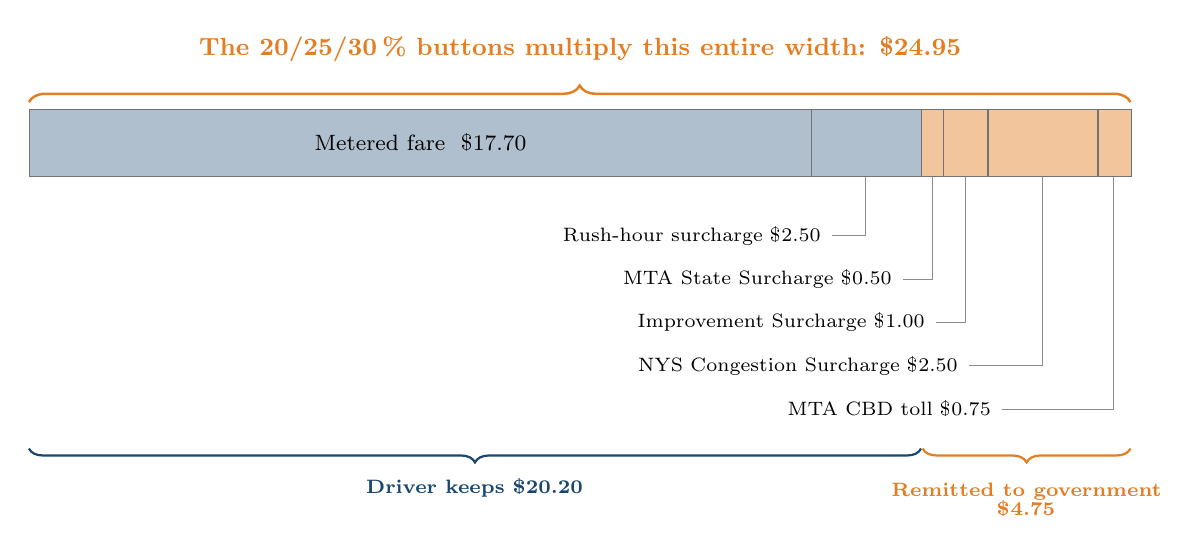
\begin{tikzpicture}[
      font=\footnotesize,
      seg/.style={draw=black!55, line width=0.5pt, minimum height=0.85cm},
      drv/.style={seg, fill=statanavy!35},
      gov/.style={seg, fill=stataorange!45},
      lab/.style={font=\scriptsize, align=center},
      lead/.style={draw=black!45, line width=0.35pt}
    ]
    % ---- scale: 0.561 cm per dollar, total $24.95 -> 14.0 cm ----
    \def\y{0}
    % segment: \seg{xstart}{width}{style}
    \node[drv, anchor=south west, minimum width=9.93cm] at (0,\y) {Metered fare \ \$17.70};
    \node[drv, anchor=south west, minimum width=1.40cm] at (9.93,\y) {};
    \node[gov, anchor=south west, minimum width=0.28cm] at (11.33,\y) {};
    \node[gov, anchor=south west, minimum width=0.56cm] at (11.61,\y) {};
    \node[gov, anchor=south west, minimum width=1.40cm] at (12.17,\y) {};
    \node[gov, anchor=south west, minimum width=0.42cm] at (13.57,\y) {};

    % ---- brace ABOVE: the tip base ----
    \draw[decorate, decoration={brace, amplitude=6pt}, stataorange, line width=0.9pt]
      (0,0.95) -- (13.99,0.95);
    \node[font=\small\bfseries, text=stataorange] at (7.0,1.62)
      {The 20/25/30\,\% buttons multiply this entire width: \$24.95};

    % ---- leader lines + labels BELOW for the narrow segments ----
    \draw[lead] (10.63,0) -- (10.63,-0.75) -- (10.20,-0.75);
    \node[lab, anchor=east] at (10.18,-0.75) {Rush-hour surcharge \$2.50};
    \draw[lead] (11.47,0) -- (11.47,-1.30) -- (11.10,-1.30);
    \node[lab, anchor=east] at (11.08,-1.30) {MTA State Surcharge \$0.50};
    \draw[lead] (11.89,0) -- (11.89,-1.85) -- (11.52,-1.85);
    \node[lab, anchor=east] at (11.50,-1.85) {Improvement Surcharge \$1.00};
    \draw[lead] (12.87,0) -- (12.87,-2.40) -- (11.94,-2.40);
    \node[lab, anchor=east] at (11.92,-2.40) {NYS Congestion Surcharge \$2.50};
    \draw[lead] (13.78,0) -- (13.78,-2.95) -- (12.36,-2.95);
    \node[lab, anchor=east] at (12.34,-2.95) {MTA CBD toll \$0.75};

    % ---- braces BELOW: who keeps it ----
    \draw[decorate, decoration={brace, mirror, amplitude=5pt}, statanavy, line width=0.8pt]
      (0,-3.45) -- (11.33,-3.45);
    \node[font=\scriptsize\bfseries, text=statanavy] at (5.66,-3.95)
      {Driver keeps \$20.20};
    \draw[decorate, decoration={brace, mirror, amplitude=5pt}, stataorange, line width=0.8pt]
      (11.35,-3.45) -- (13.99,-3.45);
    \node[font=\scriptsize\bfseries, text=stataorange, align=center] at (12.67,-4.10)
      {Remitted to government\\[-1pt]\$4.75};
  \end{tikzpicture}

  \vspace{0.9em}

  {\footnotesize
  \begin{tabular}{@{}llll@{}}
    \toprule
    Component & Amount & When it applies & Who receives it \\
    \midrule
    Metered fare            & varies & always              & \textbf{Driver} \\
    Rush-hour surcharge     & \$2.50 & weekdays 4--8pm     & \textbf{Driver} \\
    Overnight surcharge     & \$1.00 & 8pm--6am            & \textbf{Driver} \\
    \addlinespace
    MTA State Surcharge     & \$0.50 & always              & MTA \\
    Improvement Surcharge   & \$1.00 & always              & Taxi improvement fund \\
    NYS Congestion Surcharge& \$2.50 & south of 96th St    & New York State \\
    MTA CBD toll            & \$0.75 & south of 60th St    & MTA \\
    Bridge and tunnel tolls & varies & by route            & Bridge authority \\
    \bottomrule
  \end{tabular}}

  \floatnotes{Illustrative weekday 4:30pm pickup south of 60th Street in 2025;
  the metered fare is the estimation sample's pre-4pm mean. Segment widths are
  proportional to dollars. Navy components are fare revenue the driver keeps;
  orange components are collected from the rider and remitted---the driver is
  a collection agent for them and nets nothing. The rush-hour and overnight
  surcharges are set by the TLC but are \emph{not} government revenue. Every
  component, whoever receives it, sits inside the base the percentage buttons
  multiply, which is the fact this paper measures: the \$4.75 of remitted fees
  on this trip raises the suggested tip by \$0.95 at the 20 percent button, and
  raises the tip actually paid by about \$0.52 at our estimated pass-through---
  money that reaches the driver rather than the agency levying the fee.}
\end{figure}


% Illustrative diagram: how a surcharge enters the tip base.
% Institutional illustration only (permitted TikZ use); all empirical
% figures remain StataBE-generated. Amounts use the estimation sample's
% pre-4pm mean fare ($17.70) and the statutory fare stack.
\begin{figure}[!htbp]
  \centering
  \singlespacing
  \caption{\capttitle{The Mechanism on the Screen: One Trip, Four Minutes Apart}}
  \label{fig:screens}
  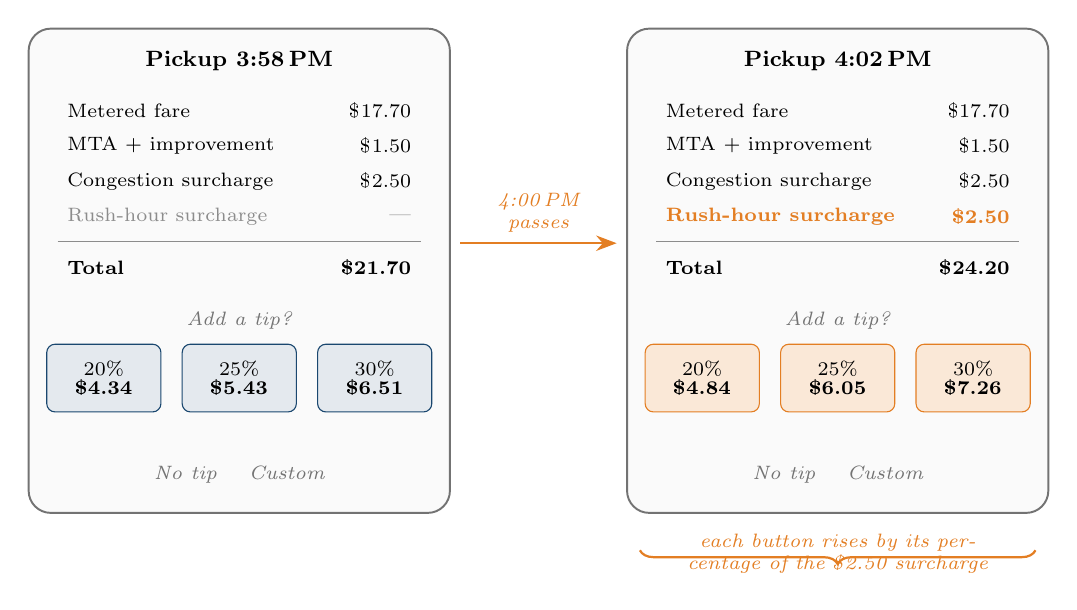
\begin{tikzpicture}[
      font=\footnotesize,
      screen/.style={rounded corners=8pt, draw=black!55, line width=0.7pt,
        fill=black!2, minimum width=5.35cm, minimum height=6.15cm},
      hdr/.style={font=\footnotesize\bfseries},
      rline/.style={font=\scriptsize},
      btn/.style={rounded corners=3pt, draw=statanavy, fill=statanavy!12,
        minimum width=1.45cm, minimum height=0.86cm, align=center,
        font=\scriptsize},
      btnhot/.style={btn, draw=stataorange, fill=stataorange!18},
      note/.style={font=\scriptsize\itshape, align=center}
    ]
    % ---------------- left screen: 3:58 PM ----------------
    \node[screen] (L) at (0,0) {};
    \node[hdr] at ($(L.north)+(0,-0.42)$) {Pickup 3:58\,PM};
    \node[rline, anchor=west] at ($(L.north west)+(0.38,-1.05)$) {Metered fare};
    \node[rline, anchor=east] at ($(L.north east)+(-0.38,-1.05)$) {\$17.70};
    \node[rline, anchor=west] at ($(L.north west)+(0.38,-1.50)$) {MTA + improvement};
    \node[rline, anchor=east] at ($(L.north east)+(-0.38,-1.50)$) {\$1.50};
    \node[rline, anchor=west] at ($(L.north west)+(0.38,-1.95)$) {Congestion surcharge};
    \node[rline, anchor=east] at ($(L.north east)+(-0.38,-1.95)$) {\$2.50};
    \node[rline, anchor=west, text=black!45] at ($(L.north west)+(0.38,-2.40)$) {Rush-hour surcharge};
    \node[rline, anchor=east, text=black!45] at ($(L.north east)+(-0.38,-2.40)$) {---};
    \draw[black!45] ($(L.north west)+(0.38,-2.72)$) -- ($(L.north east)+(-0.38,-2.72)$);
    \node[rline, anchor=west, font=\scriptsize\bfseries] at ($(L.north west)+(0.38,-3.05)$) {Total};
    \node[rline, anchor=east, font=\scriptsize\bfseries] at ($(L.north east)+(-0.38,-3.05)$) {\$21.70};
    \node[note, text=black!55] at ($(L.north)+(0,-3.72)$) {Add a tip?};
    \node[btn] (L20) at ($(L.north)+(-1.72,-4.45)$) {20\%\\[-1pt]\textbf{\$4.34}};
    \node[btn] (L25) at ($(L.north)+(0,-4.45)$) {25\%\\[-1pt]\textbf{\$5.43}};
    \node[btn] (L30) at ($(L.north)+(1.72,-4.45)$) {30\%\\[-1pt]\textbf{\$6.51}};
    \node[note, text=black!55] at ($(L.south)+(0,0.5)$) {No tip \quad Custom};
    % ---------------- right screen: 4:02 PM ----------------
    \node[screen] (R) at (7.6,0) {};
    \node[hdr] at ($(R.north)+(0,-0.42)$) {Pickup 4:02\,PM};
    \node[rline, anchor=west] at ($(R.north west)+(0.38,-1.05)$) {Metered fare};
    \node[rline, anchor=east] at ($(R.north east)+(-0.38,-1.05)$) {\$17.70};
    \node[rline, anchor=west] at ($(R.north west)+(0.38,-1.50)$) {MTA + improvement};
    \node[rline, anchor=east] at ($(R.north east)+(-0.38,-1.50)$) {\$1.50};
    \node[rline, anchor=west] at ($(R.north west)+(0.38,-1.95)$) {Congestion surcharge};
    \node[rline, anchor=east] at ($(R.north east)+(-0.38,-1.95)$) {\$2.50};
    \node[rline, anchor=west, text=stataorange, font=\scriptsize\bfseries] at ($(R.north west)+(0.38,-2.40)$) {Rush-hour surcharge};
    \node[rline, anchor=east, text=stataorange, font=\scriptsize\bfseries] at ($(R.north east)+(-0.38,-2.40)$) {\$2.50};
    \draw[black!45] ($(R.north west)+(0.38,-2.72)$) -- ($(R.north east)+(-0.38,-2.72)$);
    \node[rline, anchor=west, font=\scriptsize\bfseries] at ($(R.north west)+(0.38,-3.05)$) {Total};
    \node[rline, anchor=east, font=\scriptsize\bfseries] at ($(R.north east)+(-0.38,-3.05)$) {\$24.20};
    \node[note, text=black!55] at ($(R.north)+(0,-3.72)$) {Add a tip?};
    \node[btnhot] (R20) at ($(R.north)+(-1.72,-4.45)$) {20\%\\[-1pt]\textbf{\$4.84}};
    \node[btnhot] (R25) at ($(R.north)+(0,-4.45)$) {25\%\\[-1pt]\textbf{\$6.05}};
    \node[btnhot] (R30) at ($(R.north)+(1.72,-4.45)$) {30\%\\[-1pt]\textbf{\$7.26}};
    \node[note, text=black!55] at ($(R.south)+(0,0.5)$) {No tip \quad Custom};
    % ---------------- annotations ----------------
    \draw[-{Stealth[length=2.6mm]}, line width=0.9pt, stataorange]
      ($(L.east)+(0.12,0.35)$) -- ($(R.west)+(-0.12,0.35)$)
      node[midway, above, note, text=stataorange, text width=1.9cm]
      {4:00\,PM passes};
    \draw[decorate, decoration={brace, mirror, amplitude=5pt}, stataorange, line width=0.8pt]
      ($(R20.south west)+(-0.06,-1.75)$) -- ($(R30.south east)+(0.06,-1.75)$);
    \node[note, text=stataorange, text width=4.6cm] at ($(R.south)+(0,-0.5)$)
      {each button rises by its percentage of the \$2.50 surcharge};
  \end{tikzpicture}
  \floatnotes{Illustration of the identifying variation, using the
  estimation sample's pre-4pm mean metered fare. The two screens show the
  same trip picked up four minutes apart on a weekday. At 4:00\,PM the
  \$2.50 rush-hour surcharge (in orange) enters the total, and because
  the suggested tips are percentages of that surcharge-inclusive total,
  every button rises with it---the 20 percent button by \$0.50. Nothing
  about the ride, the driver, or the rider's intended generosity has
  changed. The paper measures how much of the surcharge reaches the
  driver through this channel: about fifteen cents per surcharge dollar,
  averaged over riders who press a button, tip a custom amount, or skip
  the tip.}
\end{figure}


\subsection{What base do the buttons use?}
Figure~\ref{fig:spikes} shows the answer before any matching exercise.
Expressed as a percentage of the all-in pre-tip total, 57.3 percent of
positive credit-card tips fall in the half-point bin at \emph{exactly}
20 percent, with further spikes at exactly 25 and 30---the three
buttons. Expressed as a percentage of the metered fare alone, the same
tips have no spikes anywhere: no bin holds more than 3.6 percent. The
smaller spikes at 10 and 15 percent of the all-in total are custom
round percentages computed on the same inclusive base---a first sign,
confirmed in Section~\ref{sec:results-vendor}, that the base governs
even riders who never press a button.

\begin{figure}[!htbp]
  \centering
  \singlespacing
  \caption{\capttitle{The Base, Drawn: The Same Tips Against Two
  Candidate Bases}}
  \label{fig:spikes}
  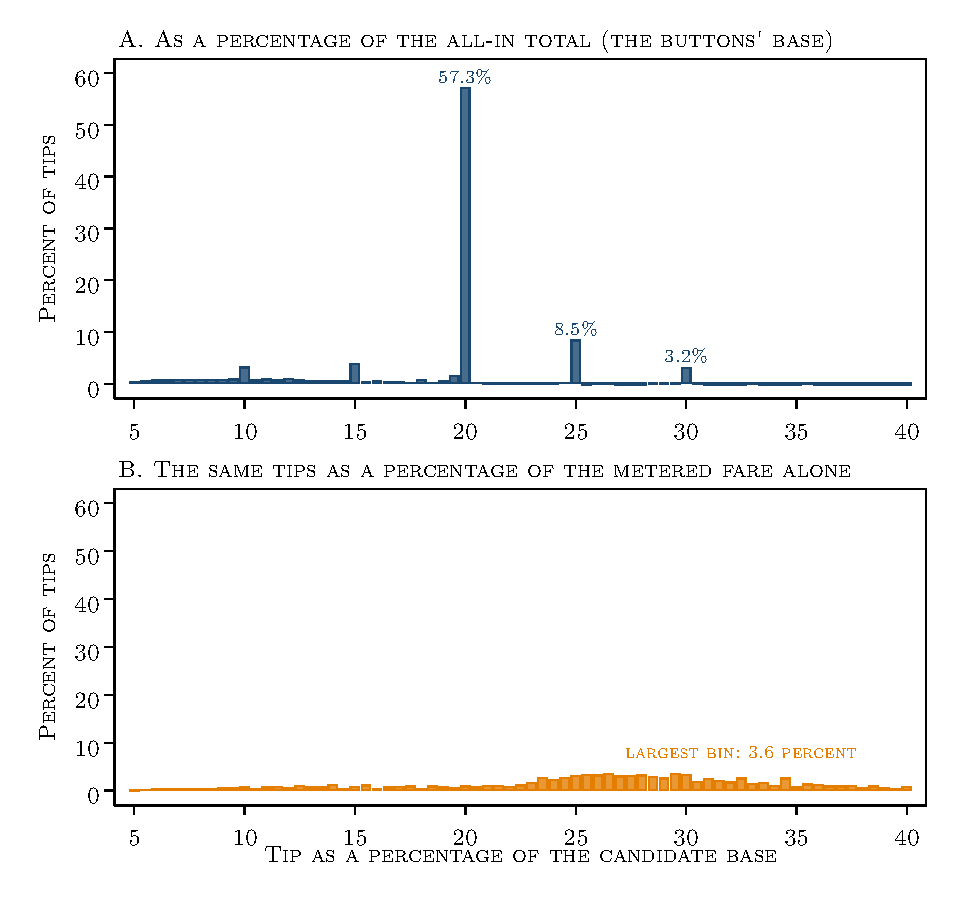
\includegraphics[width=0.88\textwidth]{fig-spikes.pdf}
  \floatnotes{June 2025, standard-rate credit-card trips with positive
  tips and no tolls (2.18 million trips), in bins of half a percentage
  point over 5--40 percent. Panel A expresses each tip as a percentage
  of the all-in pre-tip total---the base the buttons multiply;
  annotations mark the bins at exactly 20, 25, and 30 percent. Panel B
  expresses the same tips as a percentage of the metered fare alone, on
  identical axes. Only the buttons' base produces spikes.}
\end{figure}

Table~\ref{tab:vendor} sharpens the fact by vendor. For each
payment vendor we compute the share of credit-card tips that equal 20,
25, or 30 percent of a candidate base to within half a cent. In July
2024, before the CBD toll existed, the fee-inclusive and fee-exclusive
bases are numerically identical and the match rates coincide exactly, as
they must. In June 2025 they diverge sharply: the fee-inclusive total
matches 17 to 74 percent of tips depending on vendor, the fee-exclusive
total only 4 to 17 percent. All three vendors compute suggested tips on
the surcharge-inclusive total.

The table also documents striking vendor heterogeneity in adherence: at
one vendor 17 percent of tips are exact button presses, at the others 66
and 74 percent. Our estimates aggregate over this heterogeneity, so
$\rho$ should be read as a market-wide average rather than a
vendor-specific behavioral parameter.

\begin{table}[!htbp]
  \centering
  \singlespacing
  \caption{\capttitle{Which Base Do the Percentage Buttons Use?}}
  \label{tab:vendor}
  \small
  \begin{tabular}{@{}lcccc@{}}
    \toprule
    & & \multicolumn{3}{c}{Share of tips matching 20/25/30\% of:} \\
    \cmidrule(lr){3-5}
    Vendor, month & Card tips & All-in total & Excl.\ CBD fee & Fare only \\
    \midrule
    \input output/tables/tab-vendor.tex
    \bottomrule
  \end{tabular}
  \floatnotes{Card trips with positive tips and no tolls. July 2024
  precedes the CBD congestion fee, so the first two bases are identical
  by construction; June 2025 follows it. A match requires equality to
  within half a cent.}
\end{table}

\subsection{Data and estimation cells}
Trip records for every yellow-cab trip---pickup timestamp to the second,
fare components, tip (recorded for card payments only), payment type,
vendor, and pickup zone---are published monthly by the TLC
\parencite{tlc2026trip}. We aggregate to date-by-minute cells in windows
around the three clock cutoffs, recording trip counts, mean metered
surcharge, mean pre-tip total, mean card tip, the share of tips exactly
at a default button, the zero-tip share, and the card share. Separate
zone-by-fare-bin cells support the congestion-fee designs. Cells, not
raw trips, are the estimation input; the build is deterministic and
versioned with the code.

Table~\ref{tab:descriptive} describes the sample. The two surcharge
regimes are similar in composition---card share near 77 percent, mean
tips of \$3.44 and \$4.49, mean pre-tip totals of \$19 and \$26---with
the difference in the mean metered surcharge reflecting the December
2022 increase. Roughly half of all credit-card tips are exactly equal to
a default button, which is the behavioral fact the rest of the paper
builds on.

\begin{table}[!htbp]
  \centering
  \singlespacing
  \caption{\capttitle{Descriptive Statistics by Surcharge Regime}}
  \label{tab:descriptive}
  \small
  \begin{tabular}{@{}p{0.62\textwidth}r@{}}
    \toprule
    & Value \\
    \midrule
    \input output/tables/tab-descriptive.tex
    \bottomrule
  \end{tabular}
  \floatnotes{Date-by-minute cells in the estimation windows around the
  4:00pm, 8:00pm, and 6:00am cutoffs, September 2021--September 2024.
  Trip-weighted means. Tips are observed for credit-card payments only.}
\end{table}

\subsection{The motivating pattern}
Figure~\ref{fig:firststage} shows the treatment. Mean metered surcharge
by minute of day rises in a single step at 4:00pm---by \$0.72 in the
\$1.00 regime and \$1.95 in the \$2.50 regime. The step is sharp because
the surcharge is assessed on the pickup timestamp; were it assessed at
dropoff, the trip-duration distribution would smear it across half an
hour.

The steps fall short of the statutory \$1.00 and \$2.50, and the reason
is a property of the data rather than of the fare rules. The TLC's
\texttt{extra} field records miscellaneous extras, not the rush
surcharge alone, and it is contaminated on both sides of the cutoff. In
the \$2.50 regime, 23.0 percent of standard-rate card trips in the hour
\emph{before} 4:00pm already carry exactly \$2.50 in that field, while
4.5 percent of trips in the hour after carry nothing; the balance sits
at values such as \$5.00 and \$7.50 that no single surcharge explains
(Table~\ref{tab:composition}). Because the measured step is therefore
not a clean statutory dose, we report two scalings throughout: an
intention-to-treat effect per \emph{statutory} dollar, which divides by
a known constant and requires no assumption about the field, and an
instrumental-variables $\rho$ that scales by the measured step. The
first is the conservative number and the second requires the
discontinuity in \texttt{extra} to be entirely rush surcharge---an
assumption the composition table does not establish. We report both and
flag which is which at every point.

\begin{figure}[!htbp]
  \centering
  \singlespacing
  \caption{\capttitle{The First Stage: Metered Surcharge by Minute of Day}}
  \label{fig:firststage}
  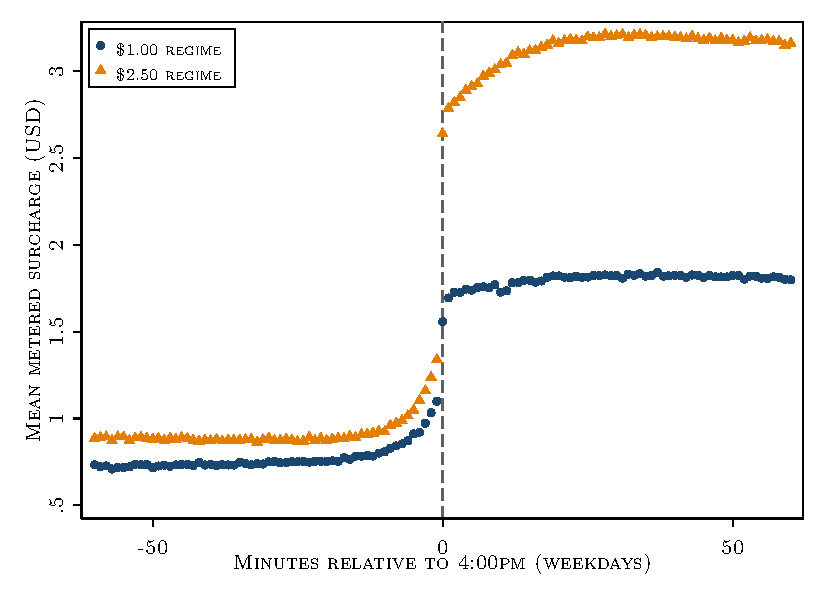
\includegraphics[width=0.82\textwidth]{fig-firststage.pdf}
  \floatnotes{Trip-weighted mean of the metered surcharge field by
  minute of pickup, weekdays excluding holidays. Navy: \$1.00 regime
  (September 2021--December 2022). Orange: \$2.50 regime (December
  2022--September 2024). The dashed line marks 4:00pm.}
\end{figure}

\begin{table}[!htbp]
  \centering
  \singlespacing
  \caption{\capttitle{What the Surcharge Field Is Made Of}}
  \label{tab:composition}
  \small
  \begin{tabular}{@{}lccccc@{}}
    \toprule
    & \multicolumn{4}{c}{Share of card trips with \texttt{extra} equal to:}
      & Mean \\
    \cmidrule(lr){2-5}
    Cutoff, side & \$0 & \$1.00 & \$2.50 & other & \texttt{extra} \\
    \midrule
    \input output/tables/tab-composition.tex
    \bottomrule
  \end{tabular}
  \floatnotes{Standard-rate card trips, weekdays excluding holidays,
  \$2.50 regime, within 60 minutes of each cutoff. The field is
  contaminated on both sides of every cutoff: a substantial share of
  trips carries the higher value before the surcharge switches on, and
  a nonzero share carries none after. This is why the measured step
  falls short of the statutory dose, and why estimates scaled by the
  measured step ($\rho^{IV}$) are reported alongside estimates scaled by
  the statutory dose (ITT).}
\end{table}


\section{Empirical Strategy}
\label{sec:model}

\subsection{Pass-through from within-day surcharge discontinuities}
Let $T_{dm}$ be the mean credit-card tip on trips picked up on date $d$
in minute-of-day $m$, $S_{dm}$ the mean metered surcharge, and $B_{dm}$
the mean pre-tip total \emph{net} of the surcharge---the metered fare and
other components. Around a clock cutoff $c$ where a surcharge switches,
with running variable $r = m - c$ and $D = \mathbf{1}\{r \ge 0\}$, we
estimate
\begin{equation}\label{eq:rd}
  T_{dm} \;=\; \alpha + \pi D + \gamma B_{dm} + f(r) + \varepsilon_{dm},
\end{equation}
with $f(r)$ local linear on each side, cells weighted by card-trip
counts, and standard errors clustered by date. Two scalings of $\pi$
appear throughout. Dividing by the \emph{statutory} dose gives the
intention-to-treat pass-through per legislated dollar, the paper's
headline estimand. Instrumenting the measured surcharge $S_{dm}$ with
$D$ gives $\rho^{IV} = \pi/\phi$, with $\phi$ the first-stage step; with
a continuous treatment this is an average causal response
\parencite{angrist1995two}, and it carries an exclusion restriction
discussed in Section~\ref{sec:results-read}.

The preferred specification differences the discontinuity of
equation~\eqref{eq:rd} against the weekend one at the same clock, where
no surcharge changes \parencite{grembi2016difference}. With $W_d$ an
indicator for weekday dates and slopes interacted with $W_d$,
\begin{equation}\label{eq:didisc}
  T_{dm} \;=\; \alpha + \pi D + \omega W_d + \delta\,(D \times W_d)
    + \gamma B_{dm} + f(r) \times W_d + \varepsilon_{dm},
\end{equation}
and $\delta$---the difference in discontinuities---divided by the
statutory dose is the headline number. Differencing removes any 4:00pm
discontinuity common to weekdays and weekends.

\subsection{Why the non-surcharge base must be controlled}
The term $\gamma B_{dm}$ is not cosmetic; it is the difference between a
credible estimate and a biased one. At 4:00pm the tip base rises by
\$2.49, of which \$1.95 is the surcharge. The remaining \$0.53 is the
non-surcharge base---chiefly the metered fare, which jumps \$0.49
because rush-hour trips are slower and dearer. Omitting $B_{dm}$
attributes those fare-driven tip increases to the surcharge and inflates
the estimate by roughly a third. Two diagnostics confirm the correction.
First, the weekend placebo---the same clock on days when no rush
surcharge exists---falls from \$0.088 to \$0.024 once $B_{dm}$ is
included, which is what a correctly specified design should do to a
placebo. Second, the corrected estimates
agree across designs that have no reason to share a bias, including one
identified purely in space (Section~\ref{sec:results-fee}). Under the
weekday--weekend difference the control is nearly redundant: dropping it
moves the estimate by about a cent (Section~\ref{sec:results}).

\subsection{Identifying assumption}
For the single difference, identification requires rider composition
and tipping norms to evolve smoothly through the clock cutoff
conditional on the fare. For the preferred difference-in-
discontinuities the requirement is weaker: whatever jumps at 4:00pm for
reasons other than the surcharge---shift changes, light, the rhythm of
the working day---must jump equally on weekends, where the clock
carries no surcharge. The residual threat is a weekday-specific,
non-surcharge discontinuity at exactly the statutory minute; placebo
cutoffs at surcharge-free minutes and a permutation over candidate
cutoffs bound it. The assumption is also checkable, and
Section~\ref{sec:results-6am} shows where it fails: at 6:00am on
weekdays the dawn compositional shift is discontinuous in precisely the
prohibited way, and the design falls apart there while its weekend twin
does not. We take the failure as evidence the diagnostics bind, not as
grounds to discard them.

\subsection{Dose, direction, and transportability}
The December 2022 increase supplies a second dose at each clock, so
comparing discontinuities across regimes tests whether one $\rho$
governs both. The within-day structure also signs the shocks: surcharges
switch \emph{on} at 4:00pm (weekdays) and 8:00pm (weekends), and the net
surcharge \emph{falls} at 8:00pm on weekdays when the rush surcharge
ends and the smaller overnight surcharge begins. Comparing upward with
downward changes tests whether pass-through is symmetric.

Finally, the 2019 New York State congestion surcharge and the January
2025 MTA congestion toll moved the same tip base at boundaries in space.
Because the fee columns exist only after each policy begins, treated
areas must be defined geographically: we learn the set of pickup zones
where each fee is actually charged from post-period incidence and apply
those zone sets to the pre-period, then estimate
difference-in-differences on zone-by-fare-bin cells with zone-fare and
month fixed effects, clustering by pickup zone. This design shares no
variation with the clock designs, so agreement between them is a
genuine out-of-sample test.


\section{Results}
\label{sec:results}

\subsection{How to read the estimates}
\label{sec:results-read}
Three numbers appear throughout this section, and they answer different
questions.

\emph{The reduced form (RF)} is the raw causal quantity: how many
dollars the average credit-card tip changes at the cutoff, holding the
non-surcharge fare constant. It is the coefficient a rider would
recognize---``tips went up 29 cents at 4:00pm.''

\emph{ITT per statutory dollar} divides the reduced form by the
\emph{statutory} surcharge change (\$2.50, \$1.00, and so on). Because
the statute is a known constant, no first stage is estimated, no
exclusion restriction is invoked, and the standard error needs no
adjustment. It answers the policy question: for each dollar the rule
adds, how much do tips rise on average across \emph{all} standard-rate
trips---including any trip the meter failed to charge? It is the
design-based number, and the one we headline.

\emph{$\rho^{IV}$} instruments the measured surcharge with the cutoff
indicator and estimates both stages jointly, so its standard error
accounts for the first stage being estimated rather than known. With a
continuous treatment it is an average causal response
\parencite{angrist1995two}, and it is causal only under an exclusion
restriction: that the entire discontinuity in the measured surcharge
field is rush surcharge. Table~\ref{tab:composition} is why that
assumption cannot be verified---the field is contaminated on both
sides of every cutoff---so we read $\rho^{IV}$ as the behavioral rate
among trips whose recorded surcharge moved, corroborated externally by
the mechanical benchmark (Appendix~\ref{app:robustness}). Which scaling
matters depends on the question: pricing a fee \emph{before} enactment
uses ITT per statutory dollar; aggregating the transfer from fees
already collected uses $\rho^{IV}$, because collections are recorded
dollars. ITT sits below $\rho^{IV}$ exactly insofar as some trips'
recorded surcharge does not move at the cutoff.

One further habit of reading: every specification conditions on the
non-surcharge base (the metered fare and fixed fees). Section
\ref{sec:results-balance} shows why this is not optional.

\subsection{What else changes at 4:00pm: balance}
\label{sec:results-balance}
Table~\ref{tab:balance} reports discontinuities in trip characteristics
at the weekday 4:00pm cutoff. The honest news first: trips themselves
change. The metered fare jumps \$0.49, trips get 0.58 miles shorter and
0.69 minutes slower---the signature of rush-hour congestion. Continuity
of trip characteristics fails, which is why we describe the design as a
\emph{fare-conditioned} within-day discontinuity rather than a
conventional regression discontinuity: identification leans on
conditioning on the fare, and on the weekend contrast, not on an
assumption that nothing else moves at 4:00pm.

What does \emph{not} change is the composition of payers: the card share
moves 0.2 percentage points and the vendor mix 0.03 points. The people
tipping on either side of the cutoff are paying the same way, through
the same machines.

\begin{table}[!htbp]
  \centering
  \singlespacing
  \caption{\capttitle{Balance at the 4:00pm Cutoff}}
  \label{tab:balance}
  \small
  \begin{tabular}{@{}lccc@{}}
    \toprule
    Trip characteristic & Pre-cutoff mean & Jump at 4:00pm & (SE) \\
    \midrule
    \input output/tables/tab-balance.tex
    \bottomrule
  \end{tabular}
  \floatnotes{Weekday standard-rate card trips, \$2.50 regime, bandwidth
  $\pm 60$ minutes, local linear, clustered by date. The fare, distance,
  and duration jumps are why every estimate in this paper conditions on
  the non-surcharge base; the null card-share and vendor-share jumps are
  why payment composition is not a confound. \sym{***}, \sym{**},
  \sym{*}: significance at 1, 5, 10 percent.}
\end{table}

\subsection{The main estimates}
Figure~\ref{fig:4pm} shows the raw pattern the estimates formalize: tips
step up at 4:00pm in both regimes, by visibly more when the surcharge is
larger, then drift down through the evening as post-rush trips shorten
and cheapen---the fare dynamics the specification conditions away.
Figure~\ref{fig:wewd} shows the same clock on weekends, where no
surcharge exists: drift without a step.

\begin{figure}[!htbp]
  \centering
  \singlespacing
  \caption{\capttitle{Credit-Card Tips by Minute Around 4:00pm}}
  \label{fig:4pm}
  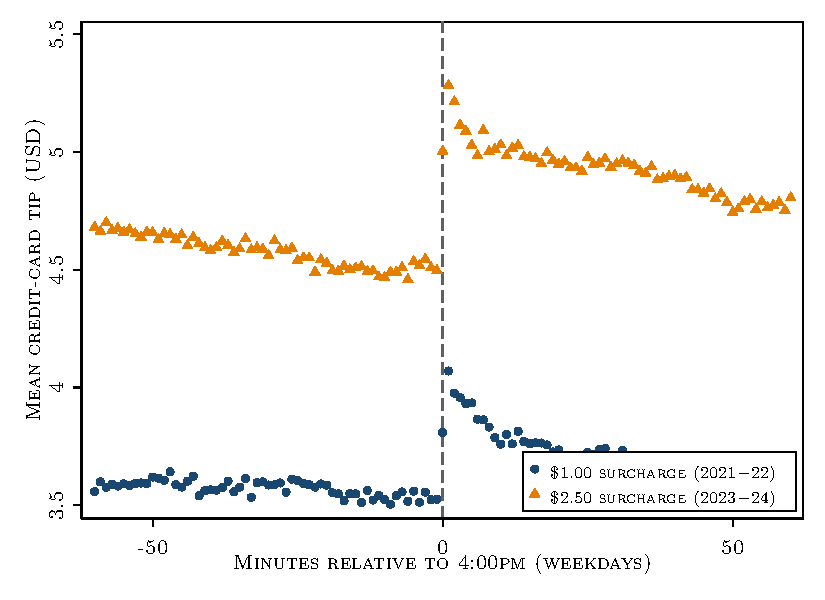
\includegraphics[width=0.86\textwidth]{fig-4pm.pdf}
  \floatnotes{Standard-rate card trips, weekdays excluding holidays,
  trip-weighted means by minute of pickup. Navy: \$1.00 regime. Orange:
  \$2.50 regime. The step at the dashed line is the treatment; the
  gradual decline afterward is rush-hour fare dynamics, absorbed by the
  fare control in estimation.}
\end{figure}

\begin{figure}[!htbp]
  \centering
  \singlespacing
  \caption{\capttitle{Weekdays Versus Weekends at the Same Clock}}
  \label{fig:wewd}
  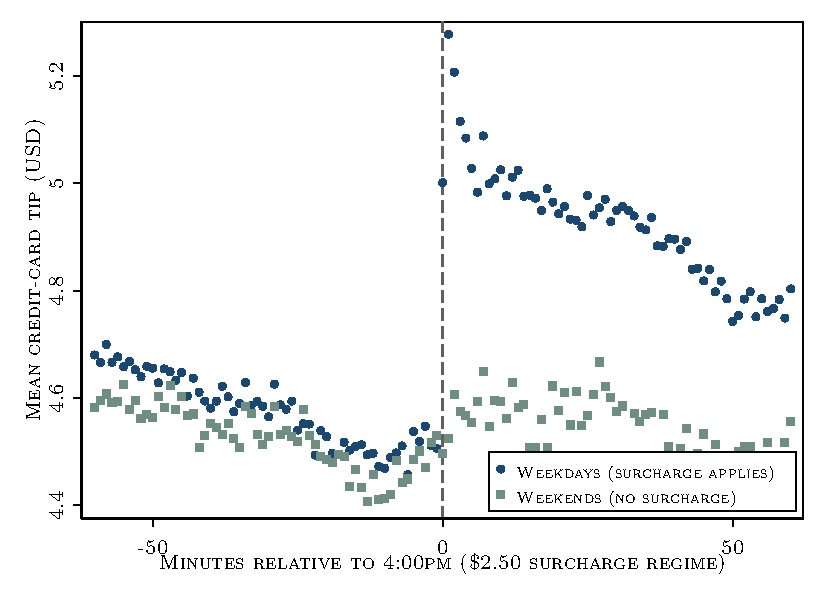
\includegraphics[width=0.80\textwidth]{fig-wewd.pdf}
  \floatnotes{Mean credit-card tips by minute around 4:00pm, \$2.50
  regime, standard-rate card trips. Weekdays (navy) receive the rush
  surcharge from 4:00pm; weekends (teal) never do.}
\end{figure}

Table~\ref{tab:main3} is the paper's central table: the same
specification at all six within-day surcharge changes, with the two
weekend placebos beneath. Reading across the top row: at the weekday
4:00pm cutoff in the \$2.50 regime, tips rise \$0.292 (SE \$0.005); per
statutory dollar that is $0.117$; instrumenting the measured surcharge,
$\rho^{IV} = 0.150$ (SE $0.002$). Reading down the $\rho^{IV}$ column is
the paper's result: $0.150$, $0.141$, $0.134$, $0.134$, $0.122$,
$0.128$. Two doses, two clocks, both directions, one parameter near
$0.14$. The placebo rows show what the same machinery finds when no
surcharge changes: \$0.024 and $-$\$0.002.

\begin{table}[!htbp]
  \centering
  \singlespacing
  \caption{\capttitle{Pass-Through at Six Surcharge Changes}}
  \label{tab:main3}
  \footnotesize
  \setlength{\tabcolsep}{4.5pt}
  \begin{tabular}{@{}lccccc@{}}
    \toprule
    & \multicolumn{2}{c}{Reduced form (USD)} & ITT per & \multicolumn{2}{c}{$\rho^{IV}$} \\
    \cmidrule(lr){2-3} \cmidrule(lr){5-6}
    Surcharge change & Tip step & (SE) & statutory \$ & Estimate & (SE) \\
    \midrule
    \input output/tables/tab-main3.tex
    \bottomrule
  \end{tabular}
  \floatnotes{Standard-rate card trips, September 2021--September 2024,
  bandwidth $\pm 60$ minutes, local linear in pickup minute, conditioning
  on the non-surcharge base, weighted by card trips, clustered by date.
  ITT divides the reduced form by the statutory dose (a known constant,
  so its SE is the RF's SE rescaled). $\rho^{IV}$ instruments the
  measured card-trip surcharge with the cutoff indicator; its SE reflects
  joint estimation of both stages. Weekend placebo rows apply the
  identical specification where no surcharge changes. \sym{***},
  \sym{**}, \sym{*}: significance at 1, 5, 10 percent.}
\end{table}

Figure~\ref{fig:coefplot} is the replication argument in one frame:
every locked change, expressed per statutory dollar, on one axis. The
six primary changes span $0.090$--$0.117$ with a precision-weighted
mean of $0.108$ (SE $0.001$). The 6:00am weekend changes sit at
$0.126$ and $0.155$ with wide intervals. The JFK flat-fare surcharge
(squares; Section~\ref{sec:results-controls}) contributes the \$4.50
and \$5.00 doses at $0.133$ and $0.149$. The 2025 congestion toll,
estimated with no clock at all, lands at $0.107$. The weekend placebos
sit at zero, and the two 6:00am weekday failures appear in grey rather
than disappearing (Section~\ref{sec:results-6am}).

\begin{figure}[!htbp]
  \centering
  \singlespacing
  \caption{\capttitle{One Parameter: Pass-Through per Statutory Dollar
  at Every Locked Change}}
  \label{fig:coefplot}
  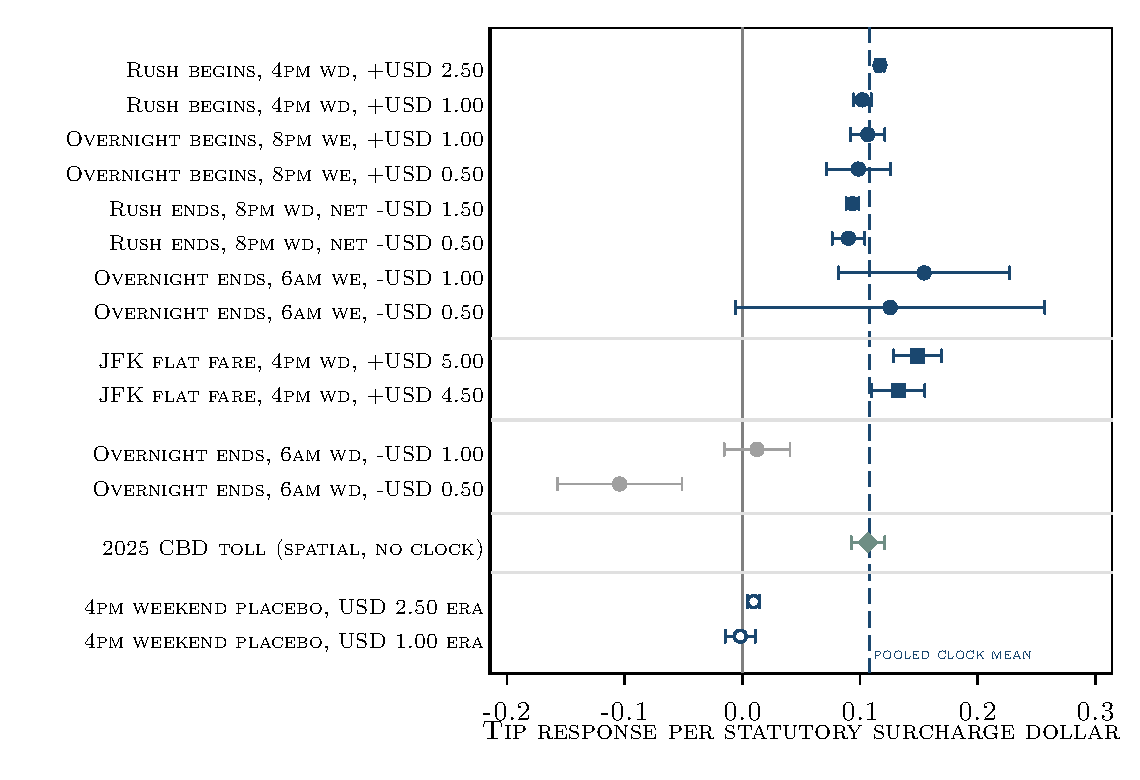
\includegraphics[width=0.94\textwidth]{fig-coefplot.pdf}
  \floatnotes{Intention-to-treat tip response per statutory surcharge
  dollar, with 95 percent confidence intervals; specification of
  Table~\ref{tab:main3} throughout. Navy circles: within-day surcharge
  changes on the standard-rate sample. Navy squares: the JFK flat-fare
  surcharge (Section~\ref{sec:results-controls}), whose higher ITT
  reflects near-complete treatment delivery (94 versus 78 percent of
  the statutory dose), not different behavior. Grey circles: the 6:00am
  weekday changes, where the dawn compositional shift breaks the fare
  conditioning (Section~\ref{sec:results-6am}). Teal diamond: the
  January 2025 congestion toll, estimated from the spatial
  origin--destination design with no clock involved, divided by the
  \$0.75 statutory toll. Hollow circles: weekend placebos at 4:00pm,
  scaled by the matched regime's dose. The dashed line marks the
  precision-weighted mean of the six primary standard-rate changes,
  $0.108$ (SE $0.001$). Minimum detectable effects (2.8 $\times$ SE)
  for the six primary changes range from $0.005$ to $0.039$ per
  statutory dollar.}
\end{figure}

Estimated as an explicit difference-in-discontinuities---the weekday
step minus the weekend step at the same clock
\parencite{grembi2016difference}, the specification of
equation~\eqref{eq:didisc}---the effect is \$0.271 (SE \$0.008) in the
\$2.50 regime and \$0.105 (\$0.008) in the \$1.00 regime: $0.108$ and
$0.105$ per statutory dollar. Dropping the fare control entirely moves
these to $0.120$ and $0.092$. The conclusion does not lean on the
functional form of the fare adjustment; the weekend difference carries
it.

The fuzzy version of the same design reports all three quantities of
the standard presentation. The first stage---the weekday--weekend
difference in the \emph{surcharge} discontinuity---is \$1.934 (SE
\$0.011) in the \$2.50 regime; the reduced form is the \$0.271 above;
and the just-identified 2SLS coefficient, instrumenting the measured
surcharge with the cutoff-by-weekday interaction, is
$\hat{\tau} = 0.140$ (SE $0.004$). In the \$1.00 regime the same three
numbers are \$0.713 (\$0.007), \$0.105 (\$0.008), and $0.147$
($0.011$): the fuzzy estimate is dose-stable, and it sits inside the
$\rho^{IV}$ family, as it must, since it differs from the single-cutoff
IV only in differencing the weekend counterfactual through both
stages.

\subsection{A working-day control, and a \$5 dose on a fare that cannot move}
\label{sec:results-controls}
Two further designs close the remaining doors on the 4:00pm result, and
both were run after the main estimates as out-of-sample checks.

\emph{Holidays.} Legal holidays are calendar weekdays on which the rush
surcharge does not apply---a working-day counterfactual that weekends
cannot supply. The federal holiday list is not the TLC list, so we
classify each holiday by its own first stage: the traditional holidays
are cleanly exempt, one observed date is partially charged and dropped,
and Juneteenth is \emph{fully charged} in all three years (first stages
of \$0.90, \$2.29, and \$2.28 against statutory doses of \$1.00 and
\$2.50)---the meters do not observe the newest federal holiday.
Differencing the weekday step against the exempt holidays gives $0.096$
per statutory dollar in the \$2.50 regime and $0.095$ in the \$1.00
regime (wild-cluster bootstrap $p < 10^{-4}$ and $p = 0.035$; holiday
clusters are few, so the bootstrap is the relevant inference)---the
same answer the weekend difference gives. And Juneteenth supplies the
converse check: a day with holiday \emph{composition} but the full
\emph{dose} shows a tip step of \$0.241 (SE \$0.067), $0.096$ per
statutory dollar. Composition off, dose on: the step follows the dose.

\emph{JFK flat fares.} The analysis plan quarantines special rate codes
from the main sample; analysed separately, the JFK flat fare is the
cleanest design in the paper. Its rush-hour surcharge is \$4.50 in the
early regime and \$5.00 after December 2022---twice the largest dose in
the main design---and it sits on a \emph{flat} fare, so the metered fare
cannot jump at 4:00pm by construction: the confound that motivates the
fare conditioning everywhere else does not exist here. The estimates
behave accordingly. The tip step is \$0.745 (SE \$0.052) at the \$5.00
dose and \$0.596 (\$0.052) at \$4.50---$0.149$ and $0.133$ per
statutory dollar---and dropping every control changes the answer by
three hundredths of a cent ($0.1486$ against $0.1489$). Weekend
placebos are null on both sides (tip $-\$0.03$ and $-\$0.05$, first
stages $-0.01$ and $-0.04$). Per \emph{recorded} surcharge dollar the
JFK estimates are $0.159$ and $0.150$, on top of the main design's
$\rho^{IV}$; the higher ITT relative to the pooled $0.108$ is treatment
delivery, not behavior---JFK meters deliver 94 percent of the statutory
dose against 78 percent on standard rates. The mechanical benchmark
tells the same story at five times the stakes: the pre-4:00pm JFK tip
rate of $17.5$ percent predicts a step of \$0.875 under complete
pass-through, and the estimate is 85 percent of it, the same fraction
as the main design. Riders tipping on an \$85 airport fare pass a \$5
surcharge into the tip at the same rate riders tipping on a \$25
Manhattan fare pass \$2.50.

Interpreting the magnitude: the average tip in this sample is 17--18
percent of the base. If riders treated a surcharge dollar exactly like a
fare dollar, complete default-mediated pass-through would put $\rho$
near $0.17$; if riders fully distinguished the surcharge---tipping on
the service, not the stack---$\rho$ would be $0$. The estimate of
$0.14$--$0.15$ says riders pass surcharges into tips at about
four-fifths of the rate they tip the fare itself: not total blindness to
the base, but close.

\subsection{Robustness}
Table~\ref{tab:bw3} shows $\rho^{IV}$ across bandwidths of 30 to 90
minutes ($0.147$--$0.156$) and donuts excluding 3, 5, or 10 minutes
around the cutoff ($0.148$--$0.152$). Because the surcharge is assessed
on the pickup time, the donut is not needed for assignment reasons; we
report it because cells adjacent to the cutoff mix minutes unevenly
within trips, and it makes no difference. Placebo cutoffs at 3:15pm and
5:00pm give tip-side effects of $-$\$0.0003 (SE \$0.007) and $-$\$0.008
(SE \$0.007)---both sides of the placebo, first stage and tip, are now
reported and both are null. A permutation over 60 candidate cutoffs,
each estimated at the same $\pm 30$ minute bandwidth as the true cutoff
and drawn only from windows that never cross 4:00pm, finds none with an
effect as large as the true cutoff's, and a wild cluster bootstrap on
the corrected reduced form rejects zero at $p < 10^{-6}$. Minimum
detectable effects---2.8 times the standard error, the analysis plan's
locked criterion---range from $0.005$ to $0.039$ per statutory dollar
across the six primary changes, so even the least-powered design could
detect an effect one-third the size of the pooled estimate.

\begin{table}[!htbp]
  \centering
  \singlespacing
  \caption{\capttitle{Bandwidth and Donut Robustness, $\rho^{IV}$}}
  \label{tab:bw3}
  \small
  \begin{tabular}{@{}lcc@{}}
    \toprule
    Specification & $\rho^{IV}$ & (SE) \\
    \midrule
    \input output/tables/tab-bw3.tex
    \bottomrule
  \end{tabular}
  \floatnotes{Weekday 4:00pm cutoff, \$2.50 regime, corrected
  specification, clustered by date. \sym{***}, \sym{**}, \sym{*}:
  significance at 1, 5, 10 percent.}
\end{table}

\subsection{The third clock: 6:00am, and where the design breaks}
\label{sec:results-6am}
The analysis plan locks a third clock. At 6:00am the overnight surcharge
\emph{ends}, so the statutory step is downward---\$0.50 before December
2022, \$1.00 after---and because the overnight surcharge applies on
every day of the week, there is no weekend placebo at this cutoff. That
absence turns out to be informative.

On weekends the estimates behave: $\rho^{IV} = 0.175$ (SE $0.041$) at
the \$1.00 dose and $0.165$ ($0.088$) at \$0.50, a little above the
main cluster but within its neighborhood. On weekdays they do not: the
\$1.00 dose gives $0.016$ ($0.018$) and the \$0.50 dose gives $-0.143$
($0.037$)---null and wrong-signed respectively.

We report this because the plan locked it, and because the pattern
diagnoses itself. The same clock and the same statutory dose produce
sensible estimates on weekends and broken ones on weekdays. What differs
between them is what happens at dawn on a working day: the pickup mix
shifts sharply toward airport-bound and commuter trips, which are longer
and dearer in a way that conditioning on the mean non-surcharge fare
does not absorb. On weekends that shift is absent and the design
recovers the same parameter as the 4pm and 8pm cutoffs. The honest
reading is that this design identifies pass-through wherever rider
composition evolves smoothly through the cutoff, and that the 6:00am
weekday window is the one place in our data where it plainly does not.
We therefore exclude the two weekday 6am estimates from the headline
range and report them here rather than in Table~\ref{tab:main3}.

\subsection{Do riders undo it?}
At the 4:00pm cutoff the share of tips exactly at a default button falls
0.85 percentage points, zero-tipping rises 0.15 points, and card use
\emph{rises} 0.19 points. Against a mechanical benchmark---the surcharge
step times the prevailing 17.4 percent tip rate---the estimated
pass-through is about nine-tenths of complete. Riders offset almost none
of the base change.

\subsection{The button is not the mechanism: vendor evidence}
\label{sec:results-vendor}
The two payment vendors offer a built-in test of \emph{how} the
pass-through operates, and it refutes our own initial hypothesis. If
pass-through worked purely through riders pressing default buttons, it
should scale with button use: Vendor 1's riders take an exact default on
19 percent of tips, Vendor 2's on 65 percent, so $\rho$ should differ
by a factor of three. It does not. Estimated separately on the same 4pm
design, $\rho^{IV} = 0.147$ (SE $0.005$) at Vendor 1 and $0.152$
($0.003$) at Vendor 2---statistically indistinguishable. Riders who
type custom amounts evidently compute their percentages on the same
fee-inclusive total the screen displays. The operative mechanism is the
\emph{base the interface presents}, not the button that presents it,
which broadens the result: redesigning buttons would not undo the
fiscal channel; redesigning the base would. Figure~\ref{fig:vendor}
shows the contrast in one frame: adherence bars that differ by a factor
of 3.5, pass-through dots that coincide.

\begin{figure}[!htbp]
  \centering
  \singlespacing
  \caption{\capttitle{Same Pass-Through, Very Different Button Use}}
  \label{fig:vendor}
  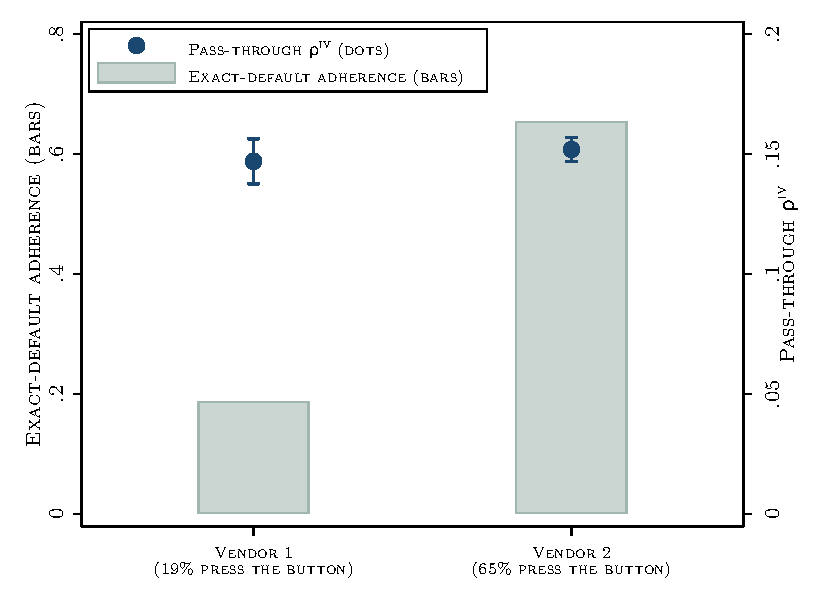
\includegraphics[width=0.76\textwidth]{fig-vendor.pdf}
  \floatnotes{Bars (right axis): share of card tips exactly at a
  default button, pre-cutoff, by payment vendor. Dots (left axis, 95
  percent CIs): $\rho^{IV}$ from the weekday 4:00pm design estimated
  separately by vendor, \$2.50 regime. If pass-through operated only
  through button presses, the dots would differ as much as the bars.}
\end{figure}

\subsection{Who passes it through}
\label{sec:results-decomp}
The mechanism has a sharper test than vendor comparisons: classify every
tip by \emph{how it was chosen}, and ask whose tips move at the cutoff.
We split card tips into four mutually exclusive types---exactly a
20/25/30 percent button, a whole-dollar amount, other custom amounts,
and zero---and estimate the weekday--weekend difference-in-
discontinuities separately for each type's mean tip and its share of
trips (Table~\ref{tab:decomp}).

If pass-through were mechanical rounding---riders nudging totals to the
nearest dollar---whole-dollar tips would carry it. They do not. In the
\$2.50 regime, button tips rise \$0.421 (SE \$0.011) and custom
non-round tips \$0.247 (\$0.027), while whole-dollar tips move \$0.043
(\$0.025). The dose comparison is more damning still: when the statutory
dose was \$1.00, button tips rose \$0.182---the response scales
one-for-one with the legislated dose---while the whole-dollar response
is \$0.04 in \emph{both} regimes, insensitive to a 150 percent dose
change. Riders who think in percentages of the displayed total pass the
surcharge through; riders who think in round dollar amounts are inert.
And nobody switches type at the cutoff: every share moves by less than
half a percentage point. The aggregate offset from complete mechanical
pass-through is not partial attention spread thinly---it is the
whole-dollar fifth of riders sitting still.

\begin{table}[!htbp]
  \centering
  \singlespacing
  \caption{\capttitle{Who Passes It Through: DiDisc by Tipping Type}}
  \label{tab:decomp}
  \small
  \begin{tabular}{@{}lccc@{}}
    \toprule
    & DiDisc & (SE) & Per statutory \$ \\
    \midrule
    \input output/tables/tab-decomp.tex
    \bottomrule
  \end{tabular}
  \floatnotes{Weekday--weekend difference-in-discontinuities at 4:00pm,
  \$2.50 regime, fare-conditioned, clustered by date; tip rows weight by
  the category's own trips, share rows by card trips. Types are mutually
  exclusive: button = tip equals 20/25/30 percent of the pre-tip total
  to within half a cent; whole-dollar = round-dollar tips not at a
  button. In the \$1.00 regime the button response is \$0.182 (0.009)
  and the whole-dollar response \$0.043 (0.027): button pass-through
  scales with the dose, whole-dollar tipping is inert at both doses.}
\end{table}

\subsection{Demand: riders do not dodge, and barely notice}
\label{sec:results-demand}
Three further margins complete the behavioral picture, and all three are
near-zero in the same direction.

\emph{No retiming.} If riders timed hails to dodge the surcharge, pickup
density would pile up before 4:00pm and hollow out after. It does not:
the share of window pickups per minute is essentially identical across
the cutoff (ten-minute ratio $0.997$ at the \$1.00 dose, $0.987$ at
\$2.50; Figure~\ref{fig:density4pm}). A 150 percent increase in the fee
produced a one percent change in timing. This doubles as the design's
sorting diagnostic: the running variable is not manipulated.

\emph{No demand response at the toll.} Log eligible trips at the January
2025 congestion boundary move $-1.0$ percent (SE $0.9$)---statistically
and economically indistinguishable from zero for a \$0.75 fee on a
\$27 ride. Combined with the tip pass-through, the driver-side ledger of
the toll is striking: drivers gain roughly \$2.2 million a year in
induced tips on eligible card trips and lose no detectable fare revenue.
At the point estimate, the congestion toll made drivers net
\emph{better} off; the confidence interval cannot exclude a net loss if
the true demand decline sits at its lower bound.

\emph{No reaction to a 150 percent surcharge increase.} On December 19,
2022 the rush surcharge jumped from \$1.00 to \$2.50 overnight. If
riders monitored their totals, percentage tipping should have dropped by
about $1.1$ points in the rush window (the fall required to keep tip
dollars fixed). Netting seasonal drift with the surcharge-free pre-rush
window, the tip rate fell $0.22$ points (SE $0.07$)---riders undid about
a fifth of the increase and passed the rest through
(Figure~\ref{fig:dec22}). That one-fifth offset independently implies
pass-through of roughly four-fifths of the prevailing tip rate, which is
precisely where the clock designs put $\rho$. And the offset is not the
start of slow learning: Figure~\ref{fig:lp-dec22} traces the response
horizon by horizon, local-projection style, for six months after the
repricing. The path settles immediately at about $-0.2$ points and
never drifts toward the $-1.1$-point full-attention benchmark. Riders
who were going to notice noticed at once; the rest never did.

\begin{figure}[!htbp]
  \centering
  \singlespacing
  \caption{\capttitle{No Delayed Learning: The Adaptation Path After December 2022}}
  \label{fig:lp-dec22}
  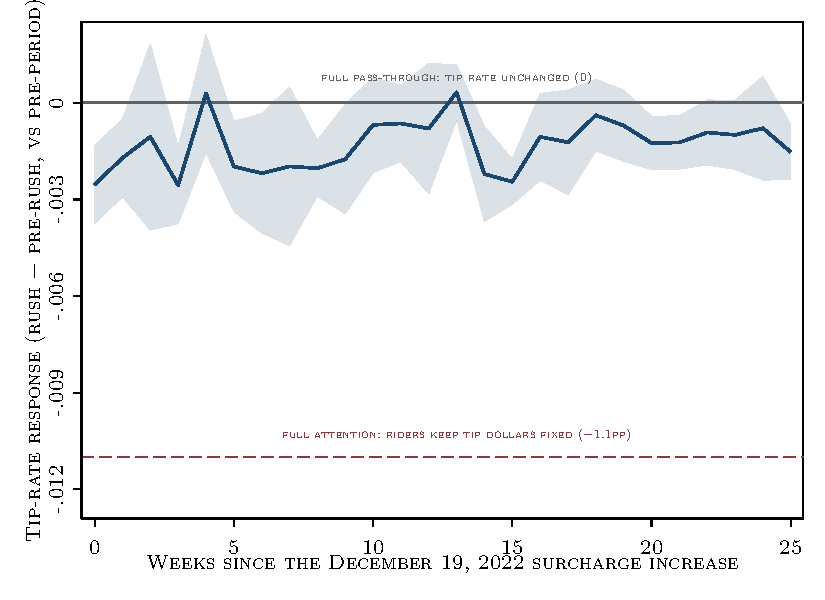
\includegraphics[width=0.82\textwidth]{fig-lp-dec22.pdf}
  \floatnotes{Weekly horizon-by-horizon responses of the rush-window
  tip rate, netted against the surcharge-free pre-rush window and
  measured relative to the 26-week pre-period mean, for 26 weeks after
  the \$1.00-to-\$2.50 repricing. The shaded band is a 95 percent
  interval from daily variation within each week. The maroon line marks
  the response that would keep tip dollars unchanged; zero marks full
  pass-through.}
\end{figure}

\begin{figure}[!htbp]
  \centering
  \singlespacing
  \caption{\capttitle{Pickup Density Through the 4:00pm Cutoff}}
  \label{fig:density4pm}
  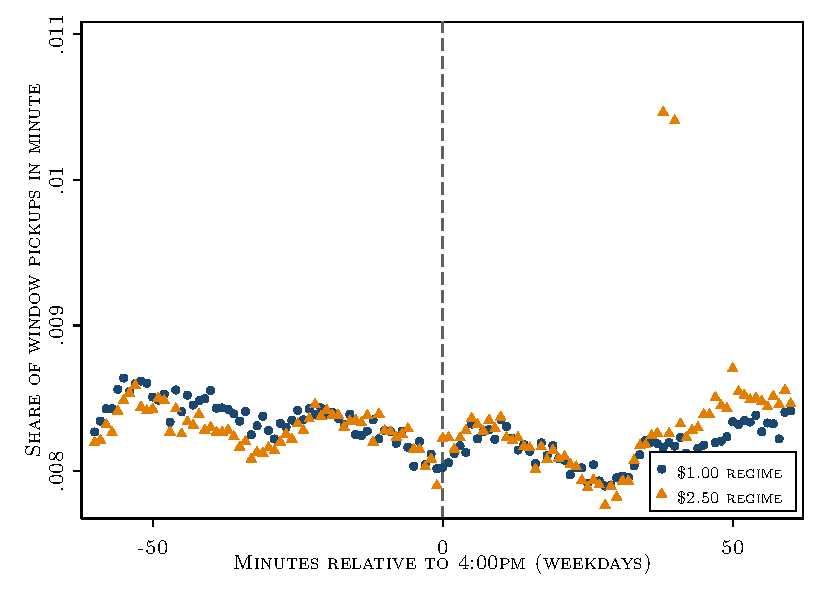
\includegraphics[width=0.78\textwidth]{fig-density4pm.pdf}
  \floatnotes{Each date's share of window pickups in each minute,
  averaged by minute, weekdays. Smooth density through the cutoff means
  riders do not retime hails around the surcharge and the running
  variable is unmanipulated.}
\end{figure}

\begin{figure}[!htbp]
  \centering
  \singlespacing
  \caption{\capttitle{The December 2022 Surcharge Increase: Did Anyone Notice?}}
  \label{fig:dec22}
  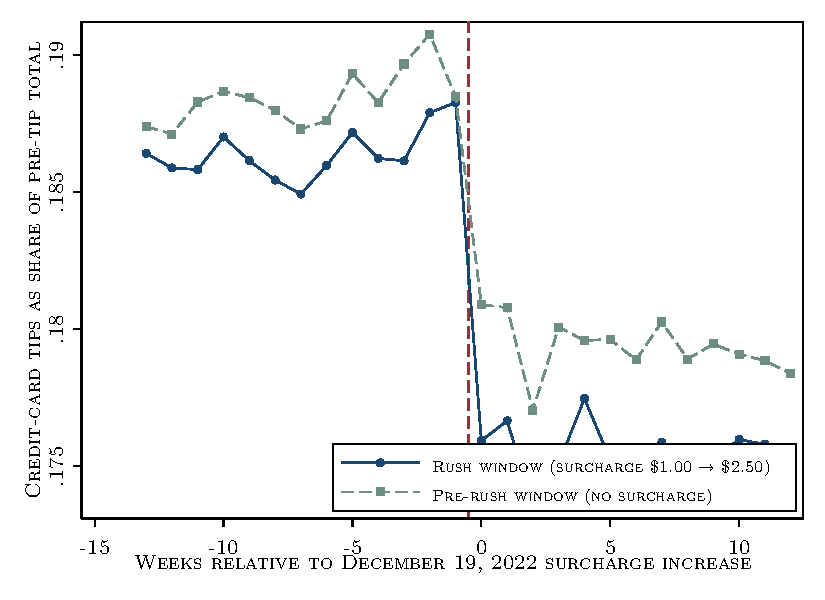
\includegraphics[width=0.80\textwidth]{fig-dec22.pdf}
  \floatnotes{Weekly mean credit-card tips as a share of the pre-tip
  total, weekdays, in the rush window (navy; surcharge rose \$1.00 to
  \$2.50 at the dashed line) and the surcharge-free pre-rush window
  (teal). Keeping tip dollars fixed would require the navy series to
  fall about 1.1 points relative to teal; it falls 0.22.}
\end{figure}

\subsection{Transportability: congestion fees}
\label{sec:results-fee}
The clock designs identify $\rho$ from surcharges that switch on a
schedule; congestion policy switches them on at boundaries in space.
The re-estimated design assigns treatment by the statutory rule---a trip
is eligible if its pickup \emph{or} dropoff lies in the fee zone---on
standard-rate card trips, and reports joint pre-trend tests. At the
January 2025 toll the origin--destination design gives a pooled tip
effect of \$0.080 (SE \$0.005) against a first stage of \$0.602 of
fee per card trip: $\rho = 0.133$ (SE $0.009$), within a cent of the
clock designs. Correcting the eligibility matters exactly as
contamination predicts: the old pickup-only assignment gave \$0.058,
because treated dropoffs sat in its control group, and its apparent
post-event fade disappears under the correct rule---post coefficients
are stable at \$0.041--\$0.052 across all six months. Two refinements
discipline the pre-period. First, seasonality: December's holiday
tipping makes any single reference month misleading, so we add
treated-by-calendar-month fixed effects, identified from a second
pre-year (2023), and measure post effects against all pre months. The
effects strengthen and stabilize---\$0.074 to \$0.089 in every one of
the six post months ($t > 8$; Figure~\ref{fig:es-fee25})---but a joint
Wald test on the 2024 pre-year against 2023 still rejects
($p = 0.0007$): treated zones genuinely drifted during 2024's recovery,
beyond seasonality. Second,
and more decisively, the eligibility rule itself supplies a
\emph{continuous dose}: the post-period share of each pickup--dropoff
pair's trips actually charged the fee, which nets out the exempt
highway corridors no geometric rule can see. Conditioning on the
non-surcharge base---the same correction the clock designs
required---the dose design yields a monotone staircase: pairs charged
up to half the time show \$0.007 (SE \$0.011), pairs charged 50--90
percent show \$0.061 ($0.015$), and pairs charged above 90 percent
show \$0.085 ($0.013$), for an implied $\rho = 0.121$. Effects that
rise step-for-step with measured treatment intensity
(Figure~\ref{fig:dose}) are difficult to attribute to zone-level
drift, which would have to reproduce the dose gradient by coincidence.

\begin{figure}[!htbp]
  \centering
  \singlespacing
  \caption{\capttitle{The Dose Staircase: Tip Effects Rise with Charging Intensity}}
  \label{fig:dose}
  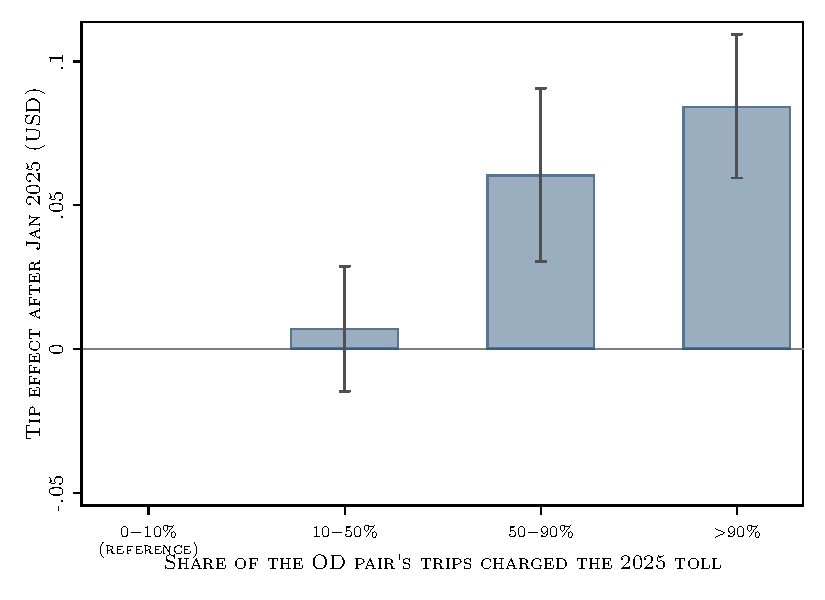
\includegraphics[width=0.76\textwidth]{fig-dose.pdf}
  \floatnotes{Post-toll tip effects by the share of each
  pickup--dropoff pair's trips actually charged the 2025 congestion
  fee (measured from post-period fee incidence), relative to pairs
  charged up to 10 percent of the time. Fare-conditioned, OD-pair and
  month fixed effects, clustered by pickup zone; bars are 95 percent
  confidence intervals.}
\end{figure} Stacking both fee adoptions into one design---each cohort with its own
unit and time effects, tips regressed on the observed fee instrumented
by eligibility-times-post, fare-conditioned throughout---yields the
\emph{average rollout effect} of putting a fee on the meter:
\[
  \bar{\rho}_{\text{rollout}} = 0.163 \ (\text{SE } 0.021).
\]
Within the same specification the cohorts are $0.171$ ($0.033$) for
2019 and $0.138$ ($0.007$) for 2025, statistically indistinguishable
($p = 0.36$). The uniform fare conditioning also resolves this
section's one outlier: the earlier 2019 estimate of $0.218$ carried
the same omitted-fare bias the clock designs taught us to remove, and
falls into line once treated identically. We still keep the spatial
evidence in a corroborating role---the binary event studies do not
pass a strict pre-trend test and we say so---while noting that the
dose gradient and the pooled rollout estimate land within two cents of
the clock designs.

\begin{table}[!htbp]
  \centering
  \singlespacing
  \caption{\capttitle{Pass-Through at Congestion Fees: The Initial
  Pickup-Only Design}}
  \label{tab:fee}
  \small
  \begin{tabular}{@{}lcccc@{}}
    \toprule
    Policy & First stage & Tip effect & (SE) & $\hat{\rho}$ \\
    \midrule
    \input output/tables/tab-fee.tex
    \bottomrule
  \end{tabular}
  \floatnotes{Zone-by-fare-bin difference-in-differences, zone-fare and
  month fixed effects, clustered by pickup zone. Windows:
  2018m7--2019m12 and 2024m1--2025m6. \emph{This is the initial
  pickup-only specification and is superseded}: it assigns treatment by
  pickup zone alone, so trips whose dropoff was in the fee zone sit in
  its control group. It is retained to show what the contamination does.
  The preferred estimates---origin--destination eligibility, fare
  conditioning, and the continuous dose---are reported in the text and
  give $\rho$ of $0.133$, $0.121$, and $0.163$ rather than the $0.146$
  and $0.254$ shown here.}
\end{table}

\begin{figure}[!htbp]
  \centering
  \singlespacing
  \caption{\capttitle{Event Study: The January 2025 Congestion Toll}}
  \label{fig:es-fee25}
  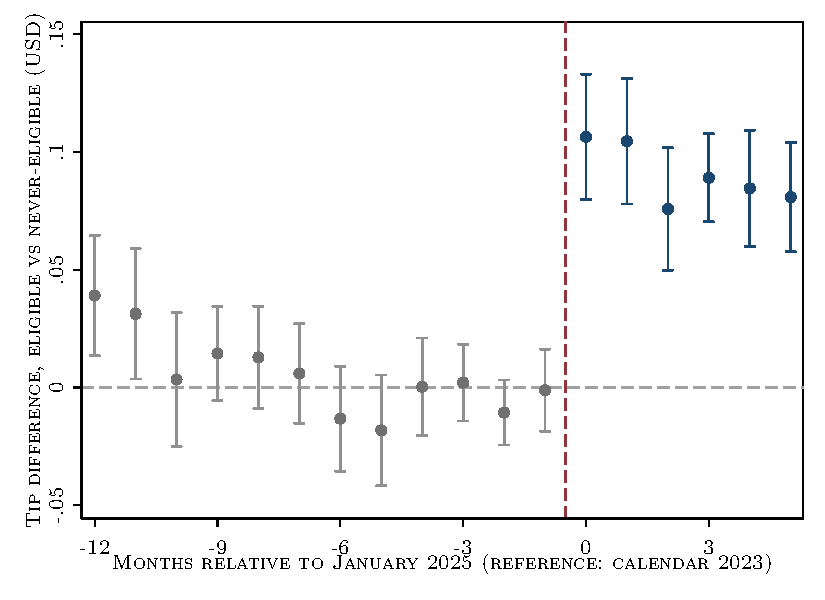
\includegraphics[width=0.78\textwidth]{fig-es-fee25.pdf}
  \floatnotes{Corrected design: origin--destination eligibility with
  treated-by-calendar-month fixed effects identified from calendar 2023;
  the twelve 2024 pre-months are shown as deviations from that seasonal
  baseline, and post coefficients are stable at \$0.074--\$0.089 with
  $t > 8$ throughout. The pre-period looks flat, and no single 2024
  coefficient is large---but a joint Wald test on all twelve rejects
  ($p = 0.0007$): treated routes drifted slightly during 2024's
  recovery. That is why the spatial evidence is read as corroboration,
  anchored by the dose gradient of Figure~\ref{fig:dose}, rather than
  as the headline. Bars: 95 percent confidence intervals.}
\end{figure}

\subsection{The size and geography of the transfer}
At $\rho = 0.15$, the \$127.2 million of 2019 congestion surcharges on
card trips implies roughly \$18.7 million of additional gratuities, and
the 2025 toll's \$17.4 million annualized implies about \$2.2 million a
year. Figure~\ref{fig:map-causal} is the spatial design's summary exhibit:
the per-zone, fare-conditioned change in tips---measured relative to
never-eligible zones---estimated at a placebo date (July 2024) and at
the real toll (January 2025), with zones muted unless significant at
five percent. At the placebo date, 6 percent of non-CBD zones and 10
percent of CBD zones show anything, scattered at random. At the real
date, \textbf{82 percent of congestion-district zones turn
significantly positive} (mean $+\$0.084$) against 18 percent
elsewhere: the tolled district materializes from the estimates alone,
with no boundary drawn. Figure~\ref{fig:map} then maps where the
resulting transfer is generated:
congestion-district pickup zones average \$46{,}000 of induced tips a
year each, against \$900 outside, so the policy boundary is visible in
the map without being drawn.

\begin{figure}[!htbp]
  \centering
  \singlespacing
  \caption{\capttitle{The Toll Appears in the Map: Placebo Versus Real Date}}
  \label{fig:map-causal}
  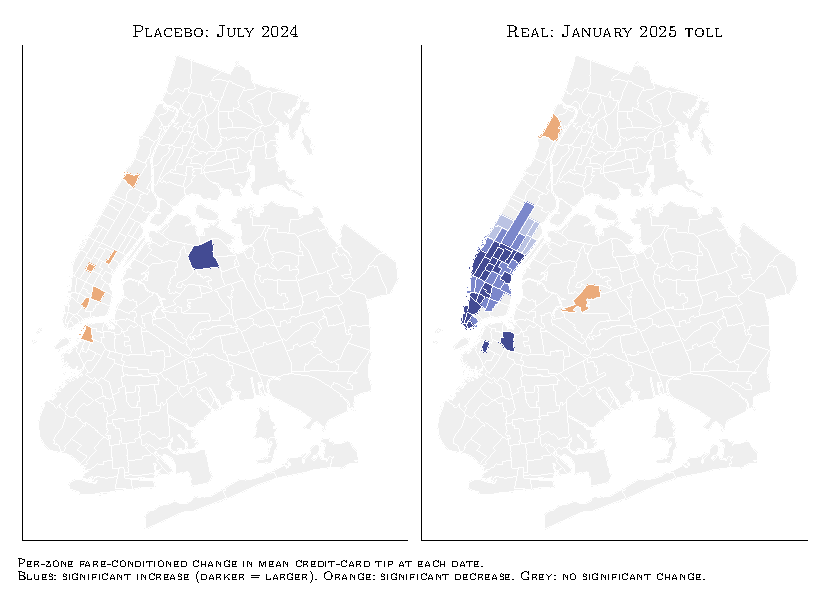
\includegraphics[width=0.98\textwidth]{fig-map-causal.pdf}
  \floatnotes{Per-pickup-zone change in mean credit-card tips,
  conditioned on fare bins and dropoff eligibility and measured relative
  to never-eligible zones, at a placebo split (July 2024, left) and the
  actual toll (January 2025, right). Blues: significant increases
  (darker larger); orange: significant decreases; grey: no significant
  change or insufficient trips. The congestion district emerges only at
  the real date.}
\end{figure}

\begin{figure}[!htbp]
  \centering
  \singlespacing
  \caption{\capttitle{Where the Transfer Is Generated}}
  \label{fig:map}
  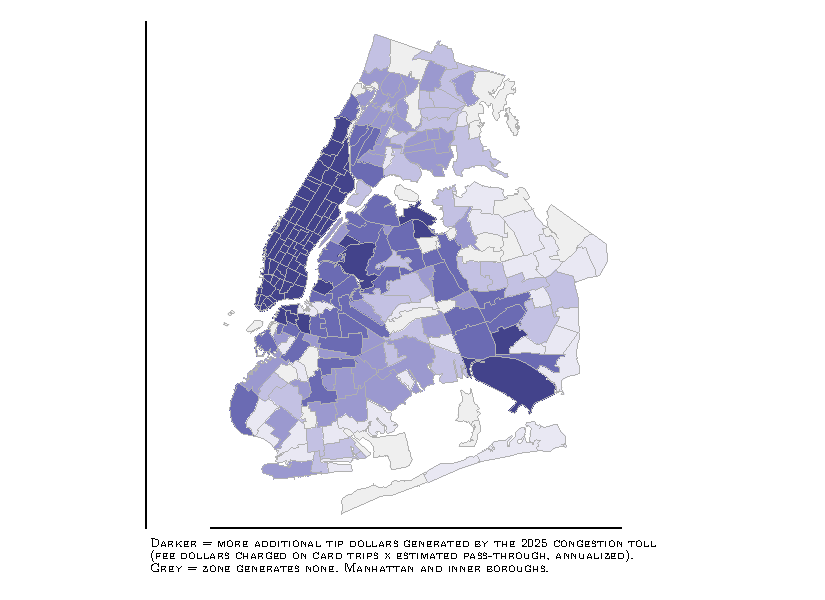
\includegraphics[width=0.80\textwidth]{fig-map.pdf}
  \floatnotes{Annualized additional tip dollars induced by the 2025
  congestion toll, by pickup taxi zone: fee dollars charged on card
  trips times the estimated pass-through. Darker = larger; grey = none.}
\end{figure}


\section{Transfer Accounting and Policy Counterfactuals}
\label{sec:counterfactuals}

The estimates support a compact transfer accounting, and its striking
feature is how little of it is assumption. Table~\ref{tab:welfare}
collects the rows.

\begin{table}[!htbp]
  \centering
  \singlespacing
  \caption{\capttitle{The Tip-Tax Ledger (USD Millions per Year)}}
  \label{tab:welfare}
  \small
  \begin{tabular}{@{}p{0.72\textwidth}r@{}}
    \toprule
    & USD m/yr \\
    \midrule
    \input output/tables/tab-welfare.tex
    \bottomrule
  \end{tabular}
  \floatnotes{Transfers are sums of observed fee payments on
  standard-rate card trips (2025 toll: 2025H1 annualized; 2019
  surcharge: calendar 2019) multiplied by the design-estimated
  pass-through. The counterfactual rows apply the dose linearity
  established across the \$0.50--\$2.50 range. The deadweight-loss bound
  is one-half times the toll times the trip decline at the lower edge of
  the demand confidence interval; the point estimate of that decline is
  indistinguishable from zero.}
\end{table}

\subsection{Transfers}
The toll moves \$16.6 million a year from riders to the MTA on card
trips---the intended, legislated flow---and \$2.2 million a year from
riders to drivers through the tip base, the unintended flow this paper
measures. The 2019 congestion surcharge, at its larger dose and volume,
moved about \$18.7 million a year through the same channel. These are
transfers, not losses: dollars change hands at face value.

\subsection{Counterfactual designs}
Because pass-through is stable in the dose from \$0.50 to \$5.00---the
JFK flat-fare surcharge supplies the \$4.50 and \$5.00 points
(Section~\ref{sec:results-controls})---the formula
$\rho \times \text{fee} \times \text{volume}$ prices design
alternatives directly. A toll set at \$2.50 would have induced roughly
\$7.4 million a year in tips. A mandated fare-only tip base---the
design one payment vendor used voluntarily in 2012
(Appendix~\ref{app:replication})---sets the induced flow to zero at no
collection cost, returning the full \$21 million a year across both
fees to riders. The tip-side of any future meter fee can be priced the
same way before enactment.

\subsection{The base-rule menu}
Because pass-through applies to whatever the base contains, every
candidate base rule has a price, and Table~\ref{tab:menu} prices the
2025 fee environment. On card trips, \$210 million a year of non-fare
dollars sit inside the tip base, generating \$23--32 million a year in
tips at the paper's two scalings. The government-remitted components
alone contribute \$141 million of base and \$15--21 million of tips---
and the largest of them is not the new CBD toll but the 2019 New York
State congestion surcharge, still running at \$2.50 per trip: \$73
million of base, \$8--11 million a year of induced tips. A regulator
choosing the base is choosing a row of this menu. Excluding the CBD
toll alone returns \$2--3 million a year to riders; excluding every
government fee returns \$15--21 million; the fare-only base that one
vendor used in 2012 returns \$23--32 million, at zero collection cost.
Tips induced by the driver-kept surcharges are a different object---a
gratuity on a price rather than on a tax---and the table labels them
separately.

\begin{table}[!htbp]
  \centering
  \singlespacing
  \caption{\capttitle{The Base-Rule Menu (USD Millions per Year, 2025
  Fee Environment)}}
  \label{tab:menu}
  \small
  \begin{tabular}{@{}p{0.52\textwidth}rcc@{}}
    \toprule
    & In tip base & \multicolumn{2}{c}{Induced tips at $\rho$ of:} \\
    \cmidrule(lr){3-4}
    Component / base rule & (USD m/yr) & $0.108$ & $0.150$ \\
    \midrule
    \input output/tables/tab-menu.tex
    \bottomrule
  \end{tabular}
  \floatnotes{Card trips, all rate codes, 2025H1 annualized. ``In tip
  base'' sums each component's dollars on card trips. Induced tips
  apply the pooled ITT per statutory dollar ($0.108$) and $\rho^{IV}$
  per recorded dollar ($0.150$); collections are recorded dollars, so
  the higher column is the aggregation-consistent one and the lower is
  conservative. Base rules give the tips returned to riders if the
  percentage buttons excluded the listed components.}
\end{table}

\subsection{Efficiency: the margins we measured are silent}
A transfer becomes a welfare problem when it distorts behavior, and on
every margin we can measure, it does not. Riders do not retime hails
around the 4:00pm surcharge (density ratio $0.99$), do not reduce
congestion-zone ridership detectably ($-1.0$ percent, SE $0.9$), do
not flee to cash (the card share rises at the cutoff), and barely
adjust tipping behavior itself (exact-default use falls under one
point). As a gauge of scale rather than a welfare bound: a Harberger
triangle computed at the unfavorable edge of the demand confidence
interval---one-half times the toll times a 2.9 percent trip
decline---comes to \$0.34 million a year, an order of magnitude below
the transfer, and the point estimate of the decline is zero. Margins we
cannot measure---whether inattentive riders would endorse the tip on
reflection, and any driver labor-supply response---are discussed below.

\subsection{What kind of transfer this is}
Two clarifications about its nature. First, on the receiving side, a
tip is the most driver-kept dollar in the fare stack: unlike metered
revenue it does not offset lease payments or commissions, so an induced
tip dollar is close to marginal driver income (net of card-processing
fees, and taxable, since card tips are recorded). The driver remits the
congestion fee itself and nets nothing on it; the induced tip is the
only part of the flow that stays. Second, the transfer is not
regulatory capture in the classic sense of an interested industry
bending rules in its favor: no beneficiary chose the base. The TLC
certifies the payment systems, so the base rule sits within the
regulable surface, but the record shows convergence by payment vendors,
not advocacy by drivers---closer to regulatory neglect than capture.
``Unlegislated'' describes a decision nobody made.

\subsection{What this accounting cannot say}
Whether the transfer harms riders depends on whether the inattentive
four-fifths would endorse the tip on reflection---a preferences
question our design-based evidence cannot answer, so we report
transfers as transfers. Driver labor supply, medallion values, and
general-equilibrium effects are likewise out of scope. The
distributional geography of the burden appears in
Section~\ref{sec:results-fee}; we label it neighborhood exposure, not
individual incidence.


\clearpage
\section{Conclusion}
\label{sec:conclusion}

New York taxi payment screens compute suggested tips as percentages of a
total that includes every government surcharge on the meter. We show
that this design choice has a measurable fiscal consequence: a
statutory dollar of surcharge raises the average credit-card tip by
about eleven cents---about fifteen cents per surcharge dollar the meter
actually records.

The estimate is well identified for a behavioral parameter of this kind.
It comes from surcharges that switch on a clock, assigned to the minute
of pickup, replicated at statutory doses from \$0.50 to \$5.00, in both
directions, at three separate times of day, against two independent
control series (weekends and exempt legal holidays), on a flat fare
where the confound cannot exist by construction (JFK),
and---crucially---reproduced by a design with no clock in it at all,
the spatial boundary of the 2025 congestion toll. Across six within-day changes the effect spans $0.090$ to
$0.117$ per statutory dollar ($\rho^{IV}$ of $0.122$--$0.150$ per
recorded dollar); the spatial estimate is $0.107$ per statutory dollar
against the clock designs' pooled $0.108$. Bandwidth and donut
variations move it by less than a cent. Two estimates, both at 6:00am on weekdays, fail, and
Section~\ref{sec:results-6am} shows why: the weekend estimates at that
same clock and dose are normal, so what breaks the weekday window is the
dawn compositional shift, not the mechanism.

Getting there required one correction we want to flag for anyone
replicating this design. The obvious specification---regress the tip on
an indicator for being past the cutoff---is badly biased, because the
metered fare jumps at 4:00pm along with the surcharge. Rush-hour trips
are slower and dearer, and part of the observed tip step is that
fare increase rather than the surcharge. Conditioning on the
non-surcharge base removes it, and the weekend placebo falls by roughly
three-quarters when it does. Designs that use time-of-day
discontinuities in prices should expect the same problem wherever the
underlying price moves with the time of day.

The interpretation is straightforward. Riders tip on a surcharge dollar
at essentially the rate they tip on a fare dollar, because the interface
gives them no way to distinguish the two. They do not switch to cash,
stop tipping, or abandon the default buttons in economically meaningful
numbers. What looks like generosity toward drivers is, at the margin,
arithmetic performed by a payment terminal.

The demand margins sharpen the picture into a single sentence: riders
do not retime hails around the 4:00pm fee, do not ride less when the
congestion toll arrives, do not switch to cash, and offset only a fifth
of a 150 percent surcharge increase---the fee is absorbed on every
margin except the one the software moves for them. It also yields a
concrete policy dial. One 2012 vendor already computed suggestions on
the fare alone, so the counterfactual is not hypothetical: mandating a
fare-only tip base would return roughly \$18.7 million a year of the 2019
surcharge's induced gratuities and \$2.2 million of the toll's to riders,
at zero collection cost, by changing one line of payment-terminal
arithmetic---about thirty cents per surcharge-paying card trip.

Two implications follow. For fiscal policy, the incidence of a fee
levied on a metered transaction does not stop at the statutory payment:
part of it continues past the agency to the worker, unlegislated and
uncounted---roughly \$18.7 million from the 2019 congestion surcharge and
\$2.2 million a year from the 2025 toll. For the growing literature on
interface-mediated payments, the result identifies a channel by which
policy and choice architecture interact: what a default is computed
\emph{on} matters as much as what it is set \emph{to}.

Three limitations bound the claims. Tips are observed only for card
payments, so the pass-through we estimate is conditional on card use,
which the design shows does not itself respond at the cutoff. Our
estimates aggregate across payment vendors whose adherence rates differ
by a factor of four, so $\rho$ is a market average rather than a
behavioral primitive. And the 2019 congestion-surcharge window predates
our minute-cell sample and abuts the pandemic; we treat it as
corroborative. Appendix~\ref{app:replication} ties the modern mechanism to the
canonical result: replicating \textcite{haggag2014default} on 2012--2013
data shows the two payment vendors of that era disagreed about the base
itself---one stopped at the fare plus surcharge, the other went on to
include tax and tolls---and that this base difference accounts for about
three-quarters of the vendor tip gap they documented. By 2025 every
vendor had converged on the inclusive base, which is what turns a
vendor-level quirk into a market-wide fiscal channel.


% ============================================================
%  BIBLIOGRAPHY
% ============================================================

\newpage
\phantomsection
\printbibliography[heading=bibintoc,title={References}]

% ============================================================
%  APPENDIX
% ============================================================

\newpage
\appendix
\appendixnumbering
\doublespacing

\section{Additional Robustness}
\label{app:robustness}

\subsection{Wild cluster bootstrap}
With 449 date clusters, cluster-robust inference on the headline
reduced form is unlikely to be distorted, but the analysis plan locks a
wild cluster bootstrap as a check. Using Webb weights and 9{,}999
replications on the \emph{corrected} weekday step in the \$2.50
regime---the preferred specification, not the uncorrected one---the
bootstrap rejects the null of no effect at $p < 10^{-6}$, with a 95
percent confidence set of $[0.2834, 0.3012]$ around a point estimate of
\$0.2923 \parencite{cameron2008bootstrap}.

\subsection{Permutation over candidate cutoffs}
The clock design has a natural randomization test: re-estimate the
discontinuity at candidate minutes where no surcharge changes and locate
the true cutoff in the resulting distribution. Every candidate---true
and placebo alike---is estimated with the same specification and the
same $\pm 30$ minute bandwidth, so the placebo distribution is
comparable to the actual statistic; candidates are drawn only from
windows that never cross 4:00pm, so no placebo inherits part of the true
discontinuity. Of 60 such candidates, \emph{none} produces an absolute
estimate as large as the true cutoff's $0.2401$.

\subsection{Placebo cutoffs}
Placebo cutoffs at 3:15pm and 5:00pm---one before the surcharge begins,
one after it is already in force---produce first stages of $-0.001$ and
$-0.023$ respectively, against $1.951$ at the true cutoff, and tip-side
effects of $-\$0.0003$ (SE \$0.0068) and $-\$0.0079$ (SE \$0.0071).
Both sides of each placebo are null. Whatever generates the 4:00pm
discontinuity is specific to the minute at which the fare schedule
changes.

\subsection{Mechanical benchmark}
A purely mechanical account of pass-through predicts a tip step equal to
the surcharge step times the prevailing tip rate on the base. In the
\$2.50 regime the surcharge step is \$1.951 and the pre-cutoff tip rate
is $0.174$, for a mechanical prediction of \$0.339. The corrected
estimate is \$0.292---about 86 percent of the mechanical benchmark. The
remaining fourteen percent is the behavioral offset: the small declines
in exact-default adherence and the small rise in zero-tipping documented
in Section~\ref{sec:results}. Pass-through is therefore close to, but
slightly below, complete.

\subsection{Synthetic difference-in-differences}
Because the binary toll event study fails a strict pre-trend test, we
re-estimate the adoption effect with synthetic difference-in-differences
\parencite{arkhangelsky2021synthetic}, which reweights both control
zones and pre-periods to match the treated group's pre-treatment
trajectory---the estimator built for exactly this failure mode. On a
balanced zone-month panel of fare-conditioned tips (treated: the 52
CBD-pickup zones; donors: never-eligible zone pools), the SDID average
treatment effect is \$0.061 (bootstrap SE \$0.050), an implied
$\rho = 0.102$---inside the family of estimates but underpowered at
zone-level aggregation, where the design surrenders the cell-level
precision of the main specifications. An in-time placebo assigning a
fake July 2024 adoption returns $-\$0.125$ (SE $0.069$), reflecting the
same 2024 drift the Wald test flags. We read SDID as corroborating the
magnitude while confirming, rather than repairing, the pre-period's
imperfection; the dose staircase remains the spatial design's strongest
evidence.

\section{Replication: Haggag and Paci (2014) and the Origins of the Base}
\label{app:replication}

\textcite{haggag2014default} established that default menus cause tips
using New York taxi data from 2009--2013, exploiting the fact that the
city's two payment vendors displayed different suggestions. We replicate
that vendor comparison on six archival months (April--June and October
2012, April--May 2013; 42.7 million credit-card trips). The two vendors
differed not only in the \emph{level} of their suggestions but in the
\emph{base} they computed them on---a fact documented independently by
\textcite{thakral2026five}, whose description of the two bases our match
rates confirm. What we add here is the arithmetic linking that base
difference to the tip gap \textcite{haggag2014default} measured.

\subsection{Recovering the menus}
Figure~\ref{fig:hp} plots the distribution of tips as a percentage of the
metered fare, by vendor, for fares of \$15 and above. Vendor 2 (VTS)
shows sharp spikes at exactly 20.0 and 25.0 percent. Vendor 1 (CMT)
shows spikes displaced slightly to the right, at 20.5 and 25.5 percent.
The displacement is not noise, and it is not a different menu level: it
is what a 20 percent button produces when the percentage is applied to a
base that includes the tax and tolls sitting on top of the fare. Vendor
2's spikes land on round percentages of the fare because its base is the
fare plus the time-of-day surcharge, and that surcharge is zero on the
majority of daytime trips---so for most of the distribution its base and
the metered fare coincide. This is exactly why the next subsection tests
the candidate bases directly rather than reading them off spike
locations: the spikes alone cannot separate ``fare'' from ``fare plus a
surcharge that is usually zero.''

\begin{figure}[!htbp]
  \centering
  \singlespacing
  \caption{\capttitle{Vendor Default Menus in the Archival Data, 2012--2013}}
  \label{fig:hp}
  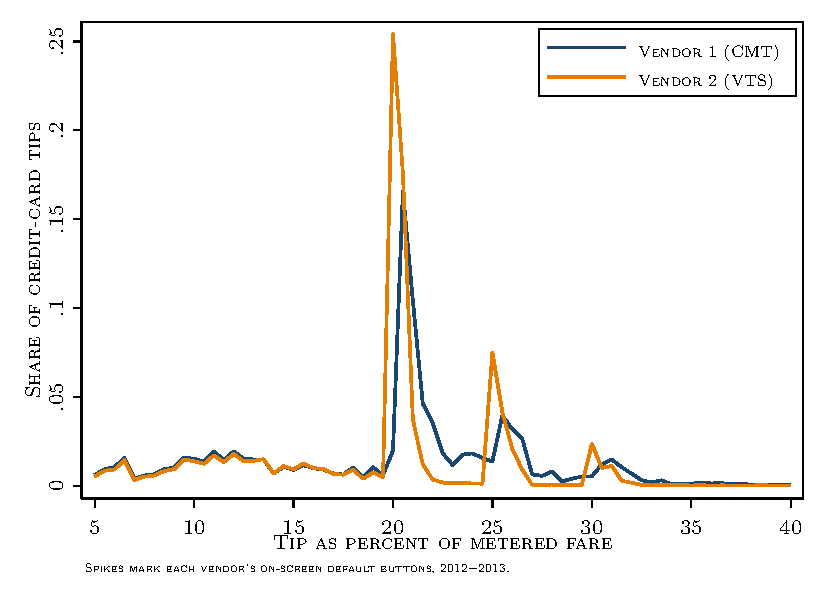
\includegraphics[width=0.84\textwidth]{fig-hp.pdf}
  \floatnotes{Distribution of credit-card tips as a percentage of the
  metered fare, in half-point bins, for trips with fares of \$15 or more.
  Spikes mark each vendor's on-screen default buttons. Vendor 2's spikes
  fall exactly on 20 and 25 percent of the fare; Vendor 1's are displaced
  upward because its percentages are computed on a surcharge-inclusive
  base.}
\end{figure}

\subsection{Testing the base directly}
Table~\ref{tab:hp-base} makes the point without reference to spike
locations. For each vendor we compute the share of positive card tips
that equal a 20, 25, or 30 percent button applied to each candidate
base, walking up the fare stack one component at a time. Testing the
full ladder matters: the surcharge field is zero on most daytime trips,
so ``fare'' and ``fare plus surcharge'' coincide there, and a test that
compares only the fare against the all-in total will appear to match the
fare for a vendor that in fact uses fare-plus-surcharge.

The pattern is categorical and identical in all six months. Vendor 2
(VTS) matches \emph{fare plus surcharge}---60.7 percent, against 30.4
percent for the fare alone and 1.4 percent for the all-in total. Vendor
1 (CMT) matches the \emph{all-in total including tax and
tolls}---53.8 percent, against essentially nothing for either narrower
base. So the vendors did not disagree about whether to include the
time-of-day surcharge; both included it. They disagreed about the sales
tax and tolls sitting above it. This is the base description in
\textcite{thakral2026five}, and our match rates confirm it.

\begin{table}[!htbp]
  \centering
  \singlespacing
  \caption{\capttitle{Which Base Did Each Vendor Use in 2012--2013?}}
  \label{tab:hp-base}
  \small
  \begin{tabular}{@{}lrcccc@{}}
    \toprule
    & & \multicolumn{4}{c}{Share of tips matching a 20/25/30\% button on:} \\
    \cmidrule(lr){3-6}
    Vendor & Card trips & Fare & $+$ surcharge & $+$ tax & $+$ tolls \\
    \midrule
    \input output/tables/tab-hp-base.tex
    \bottomrule
  \end{tabular}
  \floatnotes{Six archival months (April--June and October 2012,
  April--May 2013), credit-card trips with metered fares of \$4--60 and
  positive tips. A match requires equality to within half a cent. Each
  column adds one component of the fare stack to the base of the
  preceding column. Vendor 2 computes on fare plus surcharge; Vendor 1
  computes on the all-in total.}
\end{table}

\subsection{Does the base difference explain the tip difference?}
Vendor 1's mean tip rate is 20.6 percent of fare; Vendor 2's is 19.7
percent, an observed gap of $0.94$ percentage points. Conditioning on
month and fare bin, the gap is $0.0089$ (SE $0.0011$), reported in
Table~\ref{tab:hp}. That gap has a prediction attached to it, and the
correct prediction follows from the correct base difference: what Vendor
1 includes and Vendor 2 does not is the sales tax and tolls, which
average 6.51 percent of the metered fare. A rider pressing a 20 percent
button therefore tips $0.20 \times 0.0651 = 1.30$ percentage points of
fare more at Vendor 1 than at Vendor 2.

Not every rider presses a button. Scaling by Vendor 1's exact-default
share of 53.8 percent gives an expected gap of $0.70$ percentage
points, against an observed $0.94$. Base inclusion accounts for roughly
three-quarters of the vendor gap; the residual quarter is the level
difference in the menus themselves and the difference in zero-tipping
(2.0 percent of Vendor 1's trips against 3.6 percent of Vendor 2's).
The vendor difference that \textcite{haggag2014default} used to identify
default effects is therefore substantially---though not
wholly---attributable to the base-inclusion mechanism this paper
studies.

\begin{table}[!htbp]
  \centering
  \singlespacing
  \caption{\capttitle{Vendor Gap in Mean Tip Rate, 2012--2013}}
  \label{tab:hp}
  \small
  \begin{tabular}{@{}lc@{}}
    \toprule
    & Tip as share of fare \\
    \midrule
    \input output/tables/tab-hp.tex
    \bottomrule
  \end{tabular}
  \floatnotes{Six archival months, credit-card trips with fares of
  \$4--60. The difference conditions on month-by-fare-bin fixed effects
  and clusters by fare bin. \sym{***}, \sym{**}, \sym{*}: significance at
  1, 5, 10 percent.}
\end{table}

\subsection{Executing their deposited code}
The authors' replication archive (openICPSR 113897) contains their
cleaned 2009 analysis file and estimation code. Running their Table 2
specification verbatim on their data---the \$15 menu-threshold
discontinuity in CMT trips, third-order fare polynomial on each side,
day-of-week, hour, and borough controls, driver fixed effects, standard
errors clustered by fare bin, fares \$5--25---yields a tip jump at the
threshold of \$0.2757 (SE \$0.0060) on 6.22 million trips, with a mean
tip of \$2.22 just below the cutoff: their headline default effect,
regenerated from their archive on our machines. The lineage of the
present paper is then exact: their experiment moves the \emph{menu} at
a fare threshold and tips jump 12 percent of the base; ours moves the
\emph{base} at a clock threshold and tips move by 80 percent of the
prevailing tip rate. Both are the same object---suggested-gratuity
arithmetic doing fiscal work riders do not undo.

\subsection{Convergence}
The historical comparison closes the paper's argument. In 2012 the
market was split: one vendor stopped its base at the fare plus the
time-of-day surcharge, the other carried it all the way to the all-in
total including tax and tolls. By 2025, as Table~\ref{tab:vendor} shows,
all three vendors compute on the inclusive total. The design choice that
was once a point of disagreement between payment systems has become the
industry standard, and with it the channel through which government fees
flow into gratuities. That convergence is what makes the channel a
market-wide fiscal fact rather than one vendor's quirk, and it is the
feature of the modern setting that the archival literature could not
have observed.

\section{Data Appendix}
\label{app:empirical}

\subsection{Sources}
All trip data come from the NYC Taxi and Limousine Commission's monthly
yellow-taxi parquet files \parencite{tlc2026trip}, which cover the
universe of metered yellow-cab trips. Taxi-zone geometry comes from the
TLC's published shapefile. No restricted or proprietary data are used;
the entire analysis is reproducible from public sources with the code in
this repository.

\subsection{Cell construction}
Two builds produce the estimation inputs. The first streams each monthly
file and aggregates to date-by-minute cells within windows around the
three clock cutoffs (14:30--17:30, 18:30--21:30, and 05:00--07:00),
recording for each cell the trip count, card-trip count, mean metered
surcharge, sum of card tips, sum of card pre-tip totals, the count of
tips exactly at a 20/25/30 percent button, and the zero-tip count. The
second aggregates by month, pickup zone, and \$5 fare bin over the
congestion-fee windows (2018m7--2019m12 and 2024m1--2025m6), recording
counts, tip and base sums, and mean fee incidence. Four further
builders complete the inputs: the 6:00am window cells (the main minute
build collects only the afternoon and evening windows; the 6:00am
builder is schema-identical), the JFK flat-fare minute cells
(RatecodeID~2, all three windows, same schema), the 2012--13 vendor
base-ladder cells, and the June-2025 tip-rate histogram cells behind
Figure~\ref{fig:spikes}.

Sample restrictions are applied identically in both builds: metered
fares between \$3 and \$200, non-negative tips. Tips are recorded only
for credit-card payments, so all tip means are conditional on card use;
the card share is reported as a locked outcome at every cutoff.
Date-by-minute cells are restricted to dates within each file's own
month, which removes a small number of misdated records.

\subsection{Regime and holiday coding}
The rush-hour surcharge rose from \$1.00 to \$2.50 and the overnight
surcharge from \$0.50 to \$1.00 on December 19, 2022
\parencite{tlc2022notice}; cells are assigned to regimes on that date.
Federal and municipal holidays, on which the rush surcharge does not
apply, are excluded from weekday samples and are listed in the cleaning
code.

\subsection{Geographic treatment assignment}
The congestion-fee columns exist only after each policy takes effect, so
a treated indicator built from them would place every pre-period
observation in the control group. We therefore learn the treated zone
set from post-period fee incidence---pickup zones where the mean fee
exceeds \$0.30, giving 52 zones for the 2025 CBD toll and 115 for the
2019 surcharge---and apply that fixed zone set to the whole window.


\end{document}
